\documentclass[12pt]{report}			% Začátek dokumentu
\usepackage{MP}
\author{Martin Červený}
\title{Prostorové skenování}
\date{14. února 2022}
\vedouci{Dr.rer.nat. Michal Kočer}
\place{V~Českých Budějovicích}
\skolnirok{2021/2022}
\logo{\includegraphics[scale=1.25]{GJ8_logotyp}}
\usepackage{subcaption}
\usepackage{minted}
\begin{document}
\pagenumbering{roman}                   % číslování stránek římskými číslicemi
	\mytitlepage						% Vygenerování titulní strany

	\prohlaseni{
		Prohlašuji, že jsem tuto práci vypracoval samostatně s~vyznačením všech použitých pramenů.
	}

	\abstrakt{
          Díky rozvoji technologie se 3D skenery stávají více a~více dostupnější. Tato práce pokračuje v~popularizaci 3D skenování. Zaměřuje se na vybrané skenovací metody a~formáty souborů užívané pro uložení výsledků. Dále je zde podrobněji rozebrán návrh skenovacího postupu, který sestavuje model ze siluet předmětu. Zaměření je především na software. Konstrukce skenovacího aparátu je pouze naznačena v~příloze.

	}{
		3D skenování, STL, PLY, point cloud, mesh, siluetové skenování, C++, Python				% Klíčová slova
	}

	\podekovani{
        Rád bych poděkoval svému učiteli a~vedoucímu za užitečné rady při psaní práce. Dále pak své rodině za podporu, především Radku Trčovi, který se mnou ochotně diskutoval některé části týkající se matematiky. 			% Poděkování
	}

   {\tableofcontents\newpage}			% Obsah

\addtocounter{page}{1}		% Posunutí countru stránek
\pagenumbering{arabic}		% Číslování stránek arabskými číslicemi
	
	\chapter*{Úvod}
    
        Prostorovým skenováním přenášíme tvar předmětu do digitální podoby. Výsledný 3D objekt může být dále zkoumán či upravován prostřednictvím počítače. Rozvoj této technologie začal v~polovině 20. století. Jeho popularita vzrostla v~souvislosti s~rozmachem 3D tisku. Uplatnění nalézáme napříč mnoha obory jako je lékařství, průmysl, archeologie či jiné.

        Práce  přibližuje hlavní myšlenky některých současných metod 3D skenování a~problematiku reprezentace 3D objektů v~počítačích. Ve druhé části bylo mým cílem navrhnout metodu skenování realizovatelnou bez jakýchkoliv speciálních pomůcek. V~programu jsem se snažil vyhnout předdefinovaným knihovnám pro 3D objekty. Metodu jsem testoval na předmětech různé složitosti a~srovnával její výsledky.

        Programy jsou psány v~jazycích C++ a~Python, avšak k~pochopení popisu algoritmu není jejich znalost nutná.

	\part{Metody prostorového skenování}

		\chapter{Formáty 3D souborů}

			 Formát souboru označuje dohodnutý způsob uložení informace. Při ukládání obrázku do počítače jsou domluvena určitá pravidla. Jednou z~možností je nejdříve zapsat výšku a~šířku a~následně definovat barvu pixelů. Soubory se pak doplňují příponou, která označuje druh formátu. Výsledkem 3D skenování bude soubor, který popisuje trojrozměrný objekt.

			\section{Společná terminologie}

                Dnes existuje mnoho různých formátů. Ty nejpoužívanější mají společné znaky. Cílem je zachytit tvar povrchu předmětu. Zakřivený povrch se rozdělí do několika dvourozměrných $n$-úhelníků (polygonů), které na sebe navazují.

                Základními pojmy jsou vrcholy (\emph{vertices}), které se spojují hranami (\emph{edges}) a~tvoří plochy (\emph{faces}) polygonů. Tato struktura se označuje jako \emph{mesh}.

                \begin{figure}[h]
                    \centering
                    \includegraphics[width=9cm]{images/mesh.pdf}
                    \caption{Povrch rozložený do čtyřúhelníků}
                \end{figure}


            \section{STL}

                STL (\emph{STereoLithography}) je sice poměrně starý, avšak široce používaný formát. Poprvé byl představen již v~80. letech 20. století díky společnosti Albert Consulting Group. Svou popularitu si udržuje především kvůli stálé podpoře v~3D tisku. Plocha je fragmentována do trojúhelníků.  Setkáme se jak s~ASCII, tak s~binární podobou. \cite{all3dp}

                V~ASCII soubor začíná slovem \emph{solid}, za kterým se uvádí název souboru, popřípadě komentář. Poté následuje výpis jednoho trojúhelník za druhým. Každý je charakterizován třemi vrcholy a~normálovým vektorem stěny, který ukazuje ven z~předmětu. Na konci souboru by mělo být zapsáno \emph{endsolid}. \emph{Outer loop} bývá zvykem definovat proti směru hodinových ručiček z~pohledu zvenčí.  \cite{fabbers}

                Bohužel STL nám neumožňuje zaznamenávat nic jiného než popis povrchu předmětu. V~základní verzi není možné doplnit model o~barvy či jinou charakteristiku materiálu. \cite{sustainabilityofdigitalformats}

                V~binární podobě je princip obdobný. Po hlavičce také následuje definice trojúhelníků, vynechávají se však dělící slova jako \emph{facet normal}, \emph{outer loop} či \emph{vertex}.
                \cite{sustainabilityofdigitalformats}\cite{fabbers}



                \begin{lstlisting}[style=stlstyle]
solid ukázka zápisu STL souboru // za solid může být popis
    facet normal nx ny nz   // vektor normály trojúhelníku
        outer loop
            vertex x1 y1 z1  // souřadnice 1. vrcholu
            vertex x2 y2 z2  // souřadnice 2. vrcholu
            vertex x3 y3 z3  // souřadnice 3. vrcholu
        endloop
    endfacet
    ... // další trojúhelníky zapsané tímto stylem
endsolid
                \end{lstlisting}

                \begin{figure}[h]
                    \centering
                    \begin{subfigure}{7cm}
                        \centering
                        \includegraphics[height=5.5cm]{images/triangle.pdf}
                        \subcaption{Definice jednoho trojúhelníku}
                    \end{subfigure}
                    \hfill
                    \begin{subfigure}{7cm}
                        \centering
                        \includegraphics[height=5.5cm]{images/sphereSTL.pdf}
                        \subcaption{Reprezentace koule}
                    \end{subfigure}
                    \caption{Formát STL}
                    \label{fig:my_label}
                \end{figure}


            \section{PLY}
                PLY (\emph{Polygon File Format}) pochází ze Stanfordské univerzity, kde byl vyvinut v~90. letech 20. století. Byl používán pro zápis modelů při skenování pomocí laserové triangulace. Objekt je opět rozložen do polygonů.\cite{sustainabilityofdigitalformatsply}

                Začíná se hlavičkou, kde je popsáno, co se v~souboru dále nachází. Následuje definice vrcholů a~nakonec se zapisuje, které vrcholy tvoří $n$-úhelník. PLY nám také umožňuje model vybarvit. Každému vrcholu můžeme přiřadit jeho barvu, barva plochy polygonu je pak určena barevným přechodem mezi jeho vrcholy. \cite{ply}

                Vrcholy dostávají indexy podle pořadí, ve kterém jsou definovány, přičemž první vrchol má index 0. Indexem se na vrchol odkazujeme při zápisu polygonů.\cite{ply}

                Každý $n$-úhelník je zapsán na jedné řádce. První číslo určuje, z~kolika vrcholů je tvořen. Dále následuje výpis vrcholů v~podobě seznamu indexů. \cite{ply}

                Stejně jako v~STL existuje i~binární varianta PLY, abychom dosáhli rychlejší komunikace. \cite{sustainabilityofdigitalformatsply}

                \begin{lstlisting}[style=plystyle]
ply // začátek hlavičky
format ascii 1.0    // formát ACII nebo binární
element vertex 6    // je zde 6 vrcholů, každý má:
property float x    // x souřadnici
property float y    // y souřadnici
property float z    // z souřadnici
property uchar red  // a barvu určenou v RGB
property uchar green
property uchar blue
elemnt face 8       // následuje 8 polygonů
property list uchar int vertex_index    // jsou definovány jako indexy
                                        // vrcholů
end_header // konec hlavičky
1.000000 0.000000 0.000000 255 0 0 // 1. vrchol: x y z R G B
... // dalších 5 vrcholů
3 0 1 2 // 1. polygon: má 3 vrcholy - 0, 1 a 2
...  // dalších 7 
polygonů
                \end{lstlisting}

                \begin{figure}[h]
                    \centering
                    \begin{subfigure}{7cm}
                        \centering
                        \includegraphics[height=5.5cm]{images/trianglePLY.pdf}
                        \subcaption{Barevný přechod mezi vrcholy}
                    \end{subfigure}
                    \hfill
                    \begin{subfigure}{7cm}
                        \centering
                        \includegraphics[height=5.5cm]{images/octaeder.png}
                        \subcaption{Přechod barev na oktaedru}
                    \end{subfigure}
                    \caption{Formát PLY}
                \end{figure}

            \section{Point cloud}

                Důležitým výsledkem či mezivýsledkem procesu skenování je také tzv. mračno bodů (\emph{point cloud}). Při skenování se naměří velké množství bodů, které leží na povrchu předmětu. Každý je určen třemi souřadnicemi \emph{x}, \emph{y} a~\emph{z}. Soubor může být rozšířen dalšími specifikacemi, jako je normálový vektor k~povrchu v~daném bodě či barva bodu. Point cloud lze různými algoritmy\footnote{Např. Delaunay triangulation, alpha shapes, ball pivoting nebo marching cubes algorithm.} převést na polygonovou síť.
                Formáty pro uložení point cloudů jsou nejčastěji \verb|.dxf|, \verb|.igs|, \verb|.asc|, \verb|.vtx|, \verb|.wrl|, \verb|.obj| nebo výše popsaný \verb|.ply|. \cite{mracnobodu}\cite{pointcloud}
    
                \begin{figure}[h]
                    \centering
                    \begin{subfigure}{4cm}
                        \centering
                        \includegraphics[width=4cm]{images/pointcloud.png}
                        \subcaption{Body bez informace o~barvě \cite{pointCloudCup}}
                    \end{subfigure}
                    \hfill
                    \begin{subfigure}{9cm}
                        \centering
                        \includegraphics[width=9cm]{images/pointcloudcolor.jpg}
                        \subcaption{Body s~informací o~barvě \cite{pointCloudColor}}
                    \end{subfigure}
                    \caption{Point cloud}
                \end{figure}

                \subsection{Ball Pivoting}

                    Ball Pivoting je algoritmus pro převod point cloudu na trojúhelníkovitý mesh. Jeho vizualizace je poměrně jednoduchá. Na základě hustoty bodů zvolíme poloměr koule. Tři body tvoří trojúhelník, jestliže se jich všech koule dotýká a~zároveň neobsahuje žádný další bod uvnitř. Algoritmus začíná s~počátečním trojúhelníkem. Koule se postupně otáčí podle jedné z~hran. Tím se stále dotýká krajních bodů této hrany, a~jakmile se dotkne dalšího bodu, vytvoří se nový trojúhelník. Proces se opakuje dokud nalézáme nové body. V~nehomogenním point cloudu se algoritmus opakuje pro koule s~postupně zvětšovaným poloměrem. \cite{ballpivot}

                    \begin{figure}[h]
                            \centering
                            \includegraphics[width=12cm]{images/problematikaPivotingu.png}
                            \caption{Problematika Ball Pivotingu ve 2D. (a) Vhodně zvolený poloměr, rovnoměrná vzdálenost bodů. (b) Některé body příliš daleko, spojí se až s~větším poloměrem. (c) Příliš velký poloměr, některé body budou vynechány. \cite{ballpivot}}
                    \end{figure}

                \begin{figure}[t!bh]
                    \centering
                    \begin{subfigure}{10cm}
                        \centering
                        \includegraphics[height=5.3cm]{images/marchingCases.png}
                        \subcaption{Aproximace stěny na základě druhů vrcholů \cite{marchingCubesCases}}
                    \end{subfigure}
                    \hfill
                    \begin{subfigure}{6cm}
                        \centering
                        \includegraphics[height=5.3cm]{images/marchingCubesMesh.png}
                        \subcaption{Mesh pomocí Marching Cubes \cite{marchingCubesObr}}
                    \end{subfigure}
                    \caption{Marching Cubes algoritmus}
                \end{figure}
           
                \subsection{Marching Cubes}

                    Marching Cubes zaokrouhlí polohy bodů do 3D mřížky. Situaci si můžeme představit jako prostor složený z~malých krychliček. Vrcholy, které jsou uvnitř modelu jsou kladné, ostatní záporné. Triangulavaný mesh získáme průchodem bodů mřížky.
    
                    Jestliže jsou všechny vrcholy krychle kladné nebo všechny záporné, nejedná se o~stěnu modelu. V~opačném případě stěna prochází skrz krychli. Podle rozmístění kladných a~záporných vrcholů určíme nejlepší aproximaci stěny. Protože každý vrchol může být buď kladný, nebo záporný, dostáváme celkem $2^8$ možností. \cite{marchingCubes}

        \chapter{Metody skenování}

            3D skener je zařízení, které snímá reálný předmět. Sbírá informace především o~tvaru povrchu, případně i~barvě. Na základě naměřených dat sestrojí digitální model. Počátky 3D skenování sahají do druhé poloviny 20. století. První skenery pracovaly na principu projekce světla na předmět a~následném snímání odrazu. Dnes již známe více přístupů k~řešení problematiky 3D skenování. V~této kapitole jsou přiblíženy hlavní myšlenky nejpoužívanějších metod. \cite{uvod_do_3d_skenovani}

            \begin{figure}[h]
                \centering
                \includegraphics{Manually-operated-arm-and-strip-3D-scanner.png}
                \caption{Manuální skener promítající laserový pruh na předmět \cite{firstScanning}}
            \end{figure}

			\section{Mechanické skenování}

                Při mechanickém skenování dochází k~přímému kontaktu mezi předmětem a~skenerem. Skener je vybaven hrotem, který mechanicky přejíždí po povrchu objektu. Skener určuje souřadnice hrotu a~tvoří z~těchto bodů point cloud. \cite{mapovaniporostredi}

                V~kloubech ramene se nacházejí senzory pro určení svíraného úhlu. Tato data společně se~známými rozměry skeneru umožňují určit přesnou polohu hrotu v~prostoru. \cite{mapovaniporostredi}

                Mechanické skenování je sice přesné, avšak časově náročné, neboť musíme po předmětu jezdit ručně. Dále není možné vytvořit barevné modely nebo doplnit další charakteristiku textury. \cite{mapovaniporostredi}

                \begin{figure}[h]
                    \centering
                    \includegraphics[width=8cm]{images/mechanicalScenner.jpg}
                    \caption{Mechanický skener \cite{mechanickySkener}}
                \end{figure}

			\section{Skenování pomocí laseru}

			    Pro 3D skenování se široce využívají lasery. Cílem je opět vytvořit dostatečně hustý a~přesný point cloud. Základními dvěma principy jsou triangulace a~měření doby letu světla.

		    	\subsection{Triangulace}
    
    			    Základní schéma skeneru je znázorněno na obr. \ref{fig:triangulace}.
    			    Při měření vzdálenosti konkrétního bodu vyšleme laserový paprsek jeho směrem. Ten dopadne na skenovaný předmět a~zobrazí se do  pozorovacího senzoru -- kamery. Spojnice mezi světelným zdrojem a~senzorem se označuje jako triangulační báze. V~závislosti na vzdálenosti předmětu od triangulační báze dopadá obraz laseru do kamery pod různým úhlem. Tomuto úhlu odpovídá posun $d'$ na fotografii. \cite{triangulace1}
    
    			    Chceme-li dosáhnout přesnějšího měření, musíme soustavu postavit tak, aby malý posun $d$ odpovídal velkému posunu $d'$. Opačný přístup bychom volili při skenování větších předmětů jako jsou budovy či větší sochy. \cite{triangulace1}
    
    			    Vysílá-li laser pouze jeden paprsek, zobrazí se na předmět v~podobě tečky. Tím získáme vzdálenost pouze jednoho bodu, a~pro dosažení hustého point cloudu je proces velmi časově náročný. Proto existuje na obdobném principu 2D triangulace, kde laser vysílá rozmítaný pruh, nebo 3D triangulace, při které je vyzařován strukturovaný laserový svazek. \cite{triangulace2}
    
    			    Naměřené vzdálenosti bodů se však vždy vztahují k~triangulační bázi. Pro naskenování celého předmětu je často nutné vysílat paprsek z~různých míst. Proto jsme nuceni skenerem v~průběhu skenování pohybovat a~vždy znát jeho polohu, aby se naměřené vzdálenosti ve výsledku přepočítaly k~jednomu bodu.
    
    			    \begin{figure}[h]
                        \centering
                        \includegraphics[width=10cm]{images/triangulace.png}
                        \caption{Triangulace \cite{trinangulaceOBR}}
                        \label{fig:triangulace}
                    \end{figure}

			    \subsection{Time of flight (TOF)}

    			    Time of flight metoda je založena na konstantní rychlosti šíření světla (případně zvuku\footnote{Stejně jako světelný paprsek můžeme odrážet a~detekovat např. ultrazvuk. Zvuk však nejsme schopni zacílit na konkrétní bod jako u~laseru. Uplatněním je tak spíše detekce překážky než popis jejího tvaru.}) vzduchem. Ze světelného zdroje se vyšle světelný paprsek v~určitém úhlu pohledu směrem k~předmětu. Ten se po dopadu odráží zpět a~dopadá na světelný senzor skeneru. Skener měří časový úsek $\Delta t$ mezi okamžikem vyslání a~přijetí světelného signálu. Označme $d$ vzdálenost předmětu od skeneru. Světelný paprsek urazil za dobu $\Delta t$ dráhu $2d$. \cite{tof}

    			    $$ d=\frac{1}{2}c\Delta t$$
    
    			    Rychlost světla ve vzduchu je přibližně $\SI{3e8}{\meter\per\second}$. Po provedení jednoho výpočtu získáme vzdálenost bodu. Proces se opakuje pro několik další úhlů pohledu, popřípadě můžeme vysílat laserový paprsek z~různých míst. Výstupem je množina naměřených bodů ve formě point cloudu. \cite{tof}
    
    			    Hlavním nevýhodou je problematika měření intervalu $\Delta t$. Protože je rychlost světla za běžných podmínek veliká, vychází pro běžné vzdálenosti velmi krátký čas letu. \cite{tof}
    
    			    Například \SI{1}{\meter} urazí světlo za čas
    			    $$ t=\frac{1}{3\cdot 10^8}=\SI{3,33}{\nano\second}.$$
    
    			    Jsou tedy kladeny vysoké nároky na hardware, neboť pro kvalitní výsledky musíme dosáhnou přesnosti měření času alespoň v~řádech jednotek nanosekund.


                    \subsubsection{LiDAR}
                        Technologie, která je částečně založena na laserovém TOF, se označuje jako LiDAR (\emph{Light Detection And Rangering}). Ze zařízení je vysílán laserový paprsek, nebo spíše svazek paprsků. K~detekci vzdálenosti se využívá nejen načasování návratu paprsku, ale i~jiné fyzikální vlastnosti jako fáze odražené vlny. \cite{lidarVStof}\cite{lidarANDtof}
        
                        LiDAR nachází v~poslední době velké uplatnění. Setkáme se~s~ním např. v~moderních automobilech při řešení automatizace řízení. \cite{lidarANDtof}
        
                        Technologie LiDARU se dostává i~na nejnovější mobilní telefony, které tak zvládnou skenovat s~vysokou rychlostí i~přesností. 3D skenování se proto stává mnohem dostupnější.\cite{lidarVStof}


			\section{Fotogrametrie}
                Fotogrametrie uskutečňuje svá měření na základě několika fotografií nebo videa. Cílem je zrekonstruovat z~2D obrázků původní 3D scénu. \cite{alicevision}

                Prvním krokem je projít všechny fotografie a~nalézt mezi nimi charakteristické prvky, resp. skupiny pixelů. Nejznámější algoritmus se nazývá SIFT (\emph{Scale-invariant feature transform}).\cite{naturalfeatureextraction}

                Na základě charakteristických prvků se hledají ty fotografie, které zobrazují stejnou oblast předmětu. Charakteristické pixely každého obrázku se ukládají do datové struktury písmenkový strom na základě vzájemné podobnosti. Každý z~charakteristických prvků tak skončí v~jednom z~listů stromu. Otázka, zda se dva obrázky dívají na stejné místo, je zodpovězena porovnáním jejich písmenkových stromů.\cite{imagematching}

                V~každé dvojici obrázků, které zobrazují stejné místo, se snažíme k~sobě přiřadit všechny charakteristické prvky. Hrubou silou bychom pro každý prvek obrázku \emph{A}~našli možné odpovídající prvky obrázku \emph{B} a~podle několika kritérií vybrali nejpřesnější shodu. Největší problémy nastávají u~monotónních struktur, pak je hrubá síla velice časově náročná. Možnými optimalizacemi jsou algoritmy \emph{Přibližný nejbližší soused} nebo \emph{Kaskádové hašování}.\cite{featuresmatching}

                Nyní je vše připraveno pro hrubou rekonstrukci scény. Cílem je vypočítat mračno bodů a~umístit kamery do souřadnicového systému. Vybere se dvojice fotografií s~nejpřesnější shodou. Sobě odpovídající prvky se spojí do stop. Každá stopa by se měla stát jedním bodem point cloudu. Protože však mohlo v~předchozí kroku přiřazení dojít k~chybě, musí být některé nesouvislé stopy odstraněny. K~bodům z~prvního páru fotografií se vybere další fotografie s~nejpřesnější shodou a~přiřadí se k~současné struktuře. Každá fotografie přidá další body a~tím zpřesní celkový model. Postup se opakuje pro všechny fotografie. Následně se ještě všechny body filtrují. Protože jsme určili relativně přesné pozice a~kalibrace fotoaparátů, můžeme fotografie znovu porovnat se vzniklým point cloudem, opravit některé nepřesnosti a~vypočítat další body. \cite{structurefrommotion}

                Dalším krokem je tvorba tzv. \emph{depth maps}. Pro každý pixel fotografie určujeme jeho hloubku. Pro výpočet vybereme obrázky, na kterých je toto místo nejlépe zobrazeno. Opět je nutno filtrování výsledku, abychom předešli lokálním chybám. \cite{depthmapsestimation}

                Z~hloubkových map se generuje hustá polygonová síť. Následně se vypočítá textura objektu. Pro každý trojúhelník se hledají takové fotografie, na kterých je viditelný pod nejlepším úhlem, a~z~nich se určuje průměrná barva. \cite{meshing}\cite{texturing}

                Použití metody fotogrametrie je typické pro objekty větších rozměrů, jako jsou budovy či sochy. Oblíbená je především pro svou cenovou nenáročnost. Fotografie můžeme pořídit i~pomocí mobilního telefonu. Ke zpracování se používá např. populární open-source software Meshroom.

                \begin{figure}[h]
                    \centering
                    \includegraphics[width=15cm]{images/meshroom.png}
                    \caption{Fotogrametrie v~programu Meshroom \cite{meshroomSoftware}}
                \end{figure}

	\part{Návrh skenování pomocí fotografií siluet}


	        \section{Princip}

	            Ve své praktické části jsem navrhnul a~testoval metodu 3D skenování, která sestavuje model ze siluet předmětu. Metoda by měla být finančně nenáročná, k~její realizaci postačí v~základu počítač a~fotoaparát či mobilní telefon.

	            Skenovaný předmět se nafotí z~několika stran a~fotografie se překonvertují do formátu siluet. Při iniciaci algoritmu se v~počítači vytvoří virtuální kvádr. Na kvádr se silueta promítne z~toho místa, odkud byla fotografie pořízena. Část, kterou silueta nezasáhne, můžeme odříznout, neboť zřejmě není součástí předmětu. Po dostatečném množství odečtení siluet dostane model podobu předmětu. Nakonec promítneme fotografie na povrch meshe, čímž získá model barevnou texturu.

	            Bohužel není siluetové skenování vhodné pro všechny druhy předmětů. Na siluetách nejsme schopni zachytit dutiny. Například při skenování prázdné misky, bude výsledek odpovídat misce naplněné až po okraj.

	            Naopak výhodu je rychlost. Oproti fotogrametrii, kde musíme na výsledek čekat až několik hodin, zpracuje program siluety v~řádech několika minut. (Záleží na počtu a~rozlišení fotografií.)

                \begin{figure}[h]
                    \centering
                    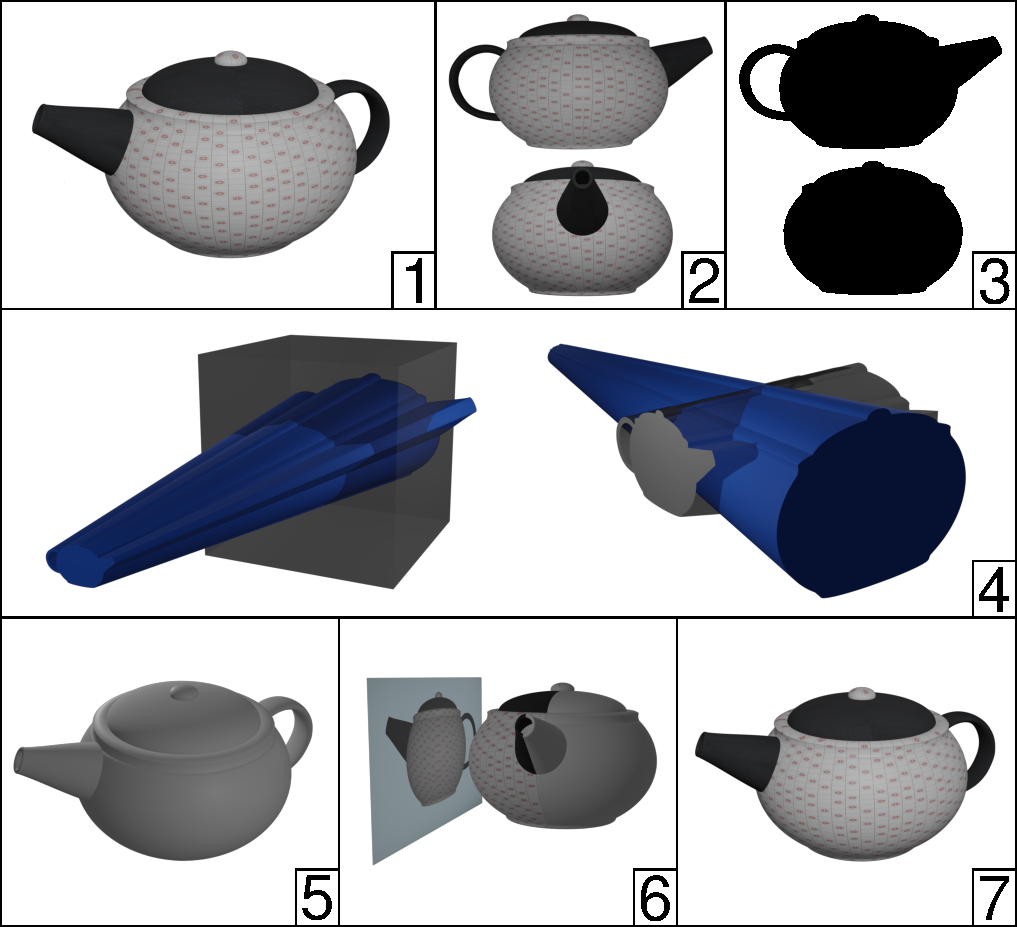
\includegraphics[width=15cm]{images/princip.pdf}
                    \caption{Princip Skenování pomocí siluet}
                \end{figure}

	            \subsection{Reprezentace v~počítači}
	                Zmíněný pomyslný kvádr představuje point cloud. Nejpřesnější je představit si kvádr složený z~mnoha malých krychliček o~jednotkové hraně. Každá krychlička je jeden bod point cloudu, její polohou myslíme souřadnice středu.

	                Siluety budeme ukládat ve formátu \verb|.pbm|. Každý pixel má hodnotu buď \verb|1|, nebo \verb|0|, podle čehož je, či není součástí modelu. Barevné fotografie uložíme ve formátu \verb|.ppm|, důvodem je především jednoduchost zápisu v~ASCII podobě.

    	    \section{Získání fotografií}

	            Přesnost procesu fotografování velice ovlivní kvalitu výsledku. Siluety musejí být na kvádr promítány přesně z~těch míst, ze kterých byly pořízeny. Abychom si usnadnili práci, umístíme kameru na fixní místo a~otáčíme skenovaným předmětem. K~otáčení je využit krokový motor NEMA 17 17HS3401, který ovládáme přes Arduino UNO a~driver L298N. Zdroj by měl mít elektromotorické napětí kolem \SI{10}{\volt}. Zároveň musí být schopen poskytovat proud do velikosti~\SI{2}{\ampere}.

                Hlavní program v~počítači řídí celý proces focení. Do Arduina je sériovou komunikací opakovaně posílán úhel, o~který se má motor otočit. Jakmile Arduino splní požadavek na otočku, je předmět vyfotografován přes externí web kameru. Fotografie se zpracuje do požadovaného formátu a~je uložena do předem zvoleného adresáře.

                Program pro Arduino je poměrně přímočarý. Pro ovládání krokového motoru je použita knihovna \verb|Stepper.h|. Neustále se kontroluje, zda nepřišla po sériové komunikaci nová zpráva. Jestliže ano, metoda \verb|step(countOfSteps)| otočí motorem o~požadovaný počet kroků. Zároveň tato metoda zastaví činnost Aruduina, dokud se motor skutečně neotočí. Nakonec Arduino odešle počítači potvrzení, že otočka je hotova, a~můžeme předmět vyfotografovat.

                Fotografie se pořizují i~zpracovávají knihovnou \verb|OpenCV|. Skenovaný předmět je postaven před pozadí jednolité barvy. Barvu každého pixelu převedeme do barevného modelu HSV (\emph{Hue, Saturation, Value}). Zadáme rozsah barvy, kterou chceme detekovat, tedy barvu pozadí. Na základě srovnání barvy každého pixelu s~rozsahem určíme, zda se jedná o~pozadí, či předmět. Můžeme tak vytvořit bitmapu reprezentující černobílou siluetu.

                Nesmíme však zapomenout uložit také původní barevný obrázek kvůli poslednímu kroku přidání textury. Abychom mohli siluety promítat na point cloud, je nutné znát informace o~pozici kamery a~úhlu otočení v~okamžiku pořízení každé fotografie \footnote{Informace promítneme do názvu souboru fotky. Chceme-li později v~programu otevřít fotografii zobrazující konkrétní část předmětu, okamžitě víme, který soubor načíst.}. Zároveň je předpokládáno (pro jednoduchost výpočtu), že kamera vždy směřuje do středu původního point cloudu tvaru kvádru.

            \section{Zpracování fotografií}

                Program je psán objektově orientovaně. Základním objektem je \verb|Point|. Dále používáme třídy \verb|PBMphoto| a~\verb|PPMphoto| pro načtení siluet a~barevných fotek. Vše spojíme v~objektu \verb|Cloud|, jehož hlavním atributem je množina všech \verb|Point|ů, které ho tvoří.

                \subsection{Point}

                    Objekt je deklarován pomocí trojice čísel -- souřadnic $x$, $y$ a~$z$ v~kartézské soustavě. Dalším atributem bodu bude jeho barva. Výchozí barvu nastavíme na černou, v~průběhu algoritmu bude přepsána. Při vyhlazování polygonové sítě budou bodům přiřazeny také vektory posunutí.

                    \subsubsection{Otáčení bodu}
                        
                        Stejně jako se otáčí předmět na skeneru, chceme být schopni otáčet i~bodem kolem libovolné přímky rovnoběžné s~osou $z$ nebo osou $x$.

                        Zaměřme se na otočení kolem přímky rovnoběžné s~osou $z$. Druhý případ dopadne analogicky. Na point cloud nahlédněme shora. Všechny body promítneme do roviny $\overleftrightarrow{xy}$. Samotná přímka se stane bodem a~problém můžeme zjednodušit na planimetrické otočení jednoho bodu okolo druhého.

                        Označme $[P_x,P_y]$ souřadnice bodu, který znázorňuje původní přímku, dále souřadnice $[Q_x,Q_y]$ bodu, kterým budeme otáčet. Úhel otočení je roven $\alpha$.

                        Pozice bodu $Q'$ po otočení je

                        $$ Q'_x = (Q_x-P_x) \cos\alpha + (Q_y-P_y) \sin\alpha + P_x$$
                        $$ Q'_y = (P_x-Q_x) \sin\alpha + (Q_y-P_y) \cos\alpha + P_y$$

                        Protože se bod otáčí kolem přímky rovnoběžné s~osou $z$, zůstane složka $z$ nezměněna. Bod je po otočení na místě $[Q'_x,Q'_y,Q_z]$.

                    \subsubsection{Průmět bodu na fotografii}

                        O~všech bodech point cloudu musíme být schopni na základě siluety rozhodnout, zda se jedná o~předmět, či nikoliv. Kamera však vytváří fotografie středovou souměrností přes objektiv. Proto i~siluetu musíme prostorem šířit na základě stejnolehlosti, jejíž střed se nachází v~místě pořízení fotografie.

                        Zaveďme zobrazení $[x,y,z]\mapsto[x,z]$ takové, že bod $[x,y,z]$ odpovídá pixelu na fotografii siluety na pozici $[x,z]$. Použijeme k~tomu pouze podobnost trojúhelníků.

                        \begin{figure}[h]
                            \centering
                            \includegraphics[width=\textwidth]{images/prumet.pdf}
                            \caption{Průmět bodu na fotografii}
                        \end{figure}

                       Pozici kamery označme $K$, bod $P$ se bude promítat do bodu $P'$.

                        $$\frac{P'_x-K_x}{K_y}=\frac{P_x-K_x}{K_y-P_y}
                        \qquad \qquad
                          \frac{P'_z-K_z}{K_y}=\frac{P_z-K_z}{K_y-P_y} 
                        $$






                \subsection{Photo}

                    Pro práci s~fotografiemi vytvoříme třídy \verb|PBMphoto| a~\verb|PPMphoto|. V~průběhu algoritmu budou využity jak siluety ve formátu \verb|.pbm|, tak originální barevné obrázky \verb|.ppm|.

                    \subsubsection{PBMphoto}
                        Formát má v~hlavičce zapsanou výšku a~šířku obrázku v~pixelech. Poté následuje výpis \verb|1| a~\verb|0|. Každá číslice pro jeden pixel -- \verb|1| pro černý a~\verb|0| pro bílý.
    
                        Objekt je iniciovaný vložením parametru typu \verb|string|, který odkazuje na místo uložení souboru fotografie v~počítači.
    
                        Jediným atributem třídy bude dvourozměrné pole, jehož velikost je dána šířkou a~výškou obrázku. Do každé buňky vložíme jednu z~hodnot proměnné \verb|boolean|.
    
                        Metodu \verb|getPixelValue(x,y)| definujeme tak, aby vracela hodnotu pixelu v~poli na souřadnicích $[x,y]$.

                    \subsubsection{PPMphoto}
                        Zde se jedná o~analogii předešlé třídy. Barva každého pixelu je však určena třemi čísly -- složkami v~modelu \emph{RGB}.
    
                        Místo typu \verb|boolean| se v buňkách nachází struktura \verb|color|, která obsahuje trojici čísel typu \verb|int| -- složky \emph{RGB}.

    	        \subsection{Cloud}

        	        Výše uvedené prvky nám usnadní sestavit point cloud. Nejdříve však ujasněme jednotky délky, které v~průběhu algoritmu použijeme. Vzdálenost je přepočítávána na pixely fotografie. Jednotková délka tak odpovídá šířce jednoho pixelu obrázku. Počáteční point cloud bude mít tvar pravidelného čtyřbokého kvádru. Rozměry přední stěny jsou totožné s~rozměry fotografie. (Nemá cenu vytvářet hustší mračno než rozlišení fotografie, řidší by však nepojalo všechny detaily.)
    
                    Hlavním atributem je pole bodů, které point cloud tvoří. V~konstruktoru pro každou celočíselnou souřadnici uvnitř kvádru vytvoříme nový bod. V~průběhu budeme přes pole bodů opakovaně iterovat a~rozhodovat, zda je bod součástí modelu, nebo zda jej smíme smazat. Odstranění prvku pole ale zabere lineární čas vzhledem k~velikosti pole. Proto raději uložíme body do datové struktury fronta. Frontou procházíme opakovaným přesouváním prvního prvku na její konec. Přesunem myslíme přidání prvního prvku na konec fronty a~následné smazání prvního členu fronty. Oboje operace mají složitost $\mathcal{O}(1)$. Body, které chceme smazat, jednoduše nepřidáme na konec fronty, pouze provedeme odstranění prvního bodu ve frontě.

                    \subsubsection{Ořezávání modelu}

                        Po iniciaci kvádru přijde řada na ořezávání. Algoritmus přesně simuluje proces focení. Kvádr otočíme na úhel, při kterém fotografie vznikla. Otočení kvádru je ekvivalentní s~otočením každého bodu kvádru. Musíme proto iterovat přes všechny body point cloudu. Při kombinaci otáčení podle více os je však nutné dodržet správné pořadí. Každý bod natočeného kvádru promítneme do roviny fotografie. Na základě pozice obrazu bodu, bude bod odstraněn, či ponechán.
    
                        Ořezávání je tedy založeno na  metodě \verb|project()| objektu \verb|Point| a~metodě \verb|getBitValue()| objektu \verb|PBMphoto|, ve kterém je uložena silueta.
    
                        Časově se jedná o~nejnáročnější proces. Musíme vzít v~potaz komunikační zdržení při načítání fotografií z~disku (přímo úměrné počtu fotografií a~jejich rozlišení). Asymptotickou složitost můžeme odhadnout na $\mathcal{O}(kn)$, kde $k$ je počet fotografií a~$n$ počet bodů point cloudu. Jelikož plánujeme zpracovat stovky fotografií a~$n$ bude v~řádech $10^7$, není rychlost příliš příznivá. Uvědomme si však, že po každém oříznutí siluety, zmenšíme počet zbývajících bodů. Následující fotografie bude proto zpracována rychleji. V~praxi se $n$ hned po několika krocích  výrazně zmenší. Časová složitost proto není tak špatná, jak naznačuje její horní odhad.

                    \subsubsection{Tvorba Meshe}

                        Body, které ve frontě zůstaly, zřejmě tvoří tvar skenovaného objektu. Dalším krokem bude sestavení polygonové sítě.
    
                        Nejprve však zdůrazněme, že se v~našem případě nejedná o~klasický point cloud. Body, které ho tvoří, totiž nereprezentují pouze povrch, nacházejí v~celém objemu předmětu. Cílem bude detekovat místo povrchu a~vytvořit v~něm odpovídající aproximaci polygonové sítě.
    
    
                        Vrátíme se k~vizualizaci původního pomyslného kvádru. Rozložili jsme ho na krychličky o~hraně velikosti pixelu. Ty krychličky, které byly vymazány, označme jako \emph{bílé}, zbylé budou \emph{černé}. Černé krychličky tvoří model skenovaného předmětu a~povrch je právě tam, kde sousedí černá krychlička s~bílou.
    
                        Vytvoříme trojrozměrné pole hodnoty \verb|boolean|. Místo černých krychliček zapíšeme \verb|1| a~místo bílých \verb|0|. Průchodem detekujeme stěny, kde se setkávají rozdílné hodnot buněk.
    
                        Nyní je mesh prakticky vytvořený, stačí zapsat nalezené stěny krychliček. Podíváme-li se na předmět z~běžného měřítka, skutečně bude věrnou kopií skenované předlohy. Jeho povrch je ovšem po přiblížení značně hrubý. Vertexy zůstaly ve mřížkových bodech a~elementární sousední polygony jsou buď ve stejné rovině, nebo svírají pravý úhel.
    
    
                        Aplikujme proto lokální úpravy k~vyhlazení. Vystouplé vrcholy nepatrně zatlačíme dovnitř předmětu, ty zapadlé naopak vytáhneme ven.
    
                        Klíčové bude určení směru posunutí vrcholu, který by vedl k~zarovnání povrchu. Zaměřme se na bod, který z~meshe příliš vyčnívá. Zarovnáme ho tak, že zatáhneme za hrany, kterými je do sítě připojen. Zobecněme tento poznatek na celý mesh. Nechť má každá hrana tendenci se smršťovat. Síla, kterou hrana působí na krajní vrcholy, přímo úměrně roste s~délkou hrany. Simulací postupného smršťování model vyhladíme.
    
                        Každému vrcholu nastavíme vektor posunutí, který je roven vektorovému součtu sousedních hran. Následně změníme polohu bodů v~odpovídajícím směru. Vzdálenost posunutí však bude pouze zlomek délky vektoru. (Nechceme tvar modelu příliš měnit, aby nedošlo ke zkreslení.) Nový povrch již bude hladší než předchozí. Metodu \verb|smoothMesh()| zavoláme několikrát po sobě k~dosažení požadované jemnosti.


                        \begin{figure}[h]
                            \centering
                            \includegraphics[width=\textwidth]{images/smoothMesh.pdf}
                            \caption{Postupné vyhlazování meshe}
                        \end{figure}

                   \subsubsection{Textura}
    
                        Posledním krokem je přidání textury. Výsledný model bude exportován ve formátu \verb|.ply|, který umožňuje definovat barvy vrcholů. Obarvování modelu tímto způsobem je vhodné pouze tehdy, je-li jeho mesh dostatečně hustý. (Náš mesh to jistě splňuje -- hustota odpovídá rozlišení fotografie.)
    
                        Informace o~barvě předmětu jsou na fotografiích formátu \verb|.ppm|. Nemusíme nutně použít všechny, avšak čím více jich zpracujeme, tím přesnější obarvení vznikne.
    
                        Postup je analogický s~ořezáváním. Pro každý bod meshe můžeme určit polohu na zvolené fotografii (metoda \verb|project()|). \verb|PPMphoto| vrací barvu pixelu v~tomto místě, kterou uložíme do atributu bodu. Oproti ořezávání však již nesmíme chápat model jako průhledný. Na fotografii není viditelný celý povrch, pouze jeho část. Zastíněné vrcholy proto  ignorujeme -- přijde na ně řada z~jiných úhlů pohledu.
    
                        Které vrcholy jsou viditelné určíme na základě vzdálenosti od místa pořízení fotografie. Vytvoříme nové trojrozměrné pole \verb|grid[][][]|, do kterého rozprostřeme body meshe. Průmětem bodu získáme souřadnice $[x,y]$ na fotografii. Bod pak vložíme do pole na pozici \verb|grid[x][y]|. Současně vypočítáme vzdálenost vkládaného bodu a~pozice kamery.
    
                        Po roztřízení iterujeme přes všechny dvojice $[i,j]$ v~rozsahu šířky a~výšky fotografie. Nahlédneme na body, jejichž průmětem je právě tato poloha. Viditelný je zřejmě bod z~pole \verb|grid[i][j]|, který je nejblíže ke kameře, proto mu zapíšeme barvu pixelu $[i,j]$.
    
                        Stále však přehlížíme vlastnosti metody \verb|project()|. Souřadnice promítnutého bodu nejsou vždy celočíselné a~poloha je tak zaokrouhlena na nejbližší pixel. Proto mohou nastat následující situace:

                        \begin{enumerate}
                            \item Sousední viditelné body spadnou na stejné místo \verb|grid[i][j]|.
                            \item Některá pole \verb|grid[i][j]| zůstanou prázdná.
                            \item Do pole \verb|grid[i][j]| nezasáhne žádný bod viditelného povrchu, některé body zastíněného sem ale spadnou.
                            \end{enumerate}
    
                        Rozhodnutí o~viditelnosti bodu proto rozšíříme o~další dvě pravidla.
                        \begin{itemize}
                            \item Neobarvíme pouze nejbližší bod z~\verb|grid[i][j]|, ale i~ostatní, jejichž vzdálenost se od té nejmenší tolik neliší (Řešení problému 1.)
                            \item Na pozici $[i,j]$ nebereme v~potaz pouze nejmenší vzdálenost pole \verb|grid[i][j]|, ale i~vzdálenosti na okolí (o~poloměru několika jednotek pixelů). Bude-li některá z~nich výrazně nižší, nebude bod obarven i~přes svou nejnižší vzdálenost v~rámci \verb|grid[i][j]|. (Řešení problému 3.)
                        \end{itemize}

                        Metoda \verb|color()| je volána na více fotografií z~různých úhlů pohledu. Viditelné povrchy se na nich překrývají, proto by vrcholy byly vybarveny vícekrát. Na každé z~fotografií mohl být předmět jinak osvícen, výsledná barva bude průměrem\footnote{Barvu zapisujeme v~modelu \emph{RGB}, průměr definujme jako aritmetický průměr jednotlivých složek.} barev z~fotografií, na kterých je vrchol viditelný.



    	    \section{Troubleshooting}

    	        Podle předpokladů algoritmu měla osa otáčení předmětu splývat s~vertikální osou fotografie. Tento požadavek však nebylo snadné dokonale splnit, docházelo k~odchylce v~řádech jednotek pixelů. Relativně malá odchylka však způsobila podstatnou deformaci výsledku.

    	        Proto byl program upraven následujícím způsobem. Každé sérii fotografií přidáme textový soubor, který ukládá informace o~skutečné pozici středu otáčení a~kamery. Oba body nakalibrujeme na základě průběžných výsledků -- např. zarovnáváním protějších siluet viz \ref{delataceSiluet}.

              \begin{figure}[h]
                    \centering
                    \begin{subfigure}[b]{0.3\textwidth}
                     \centering
                     \includegraphics[width=\textwidth]{images/skutecnyPredmet.png}
                     \caption{Skutečný vzor}
                    \end{subfigure}
                    \hfill
                    \begin{subfigure}[b]{0.3\textwidth}
                     \centering
                     \includegraphics[width=\textwidth]{images/posunuteSiluety.png}
                     \caption{Posun 3D siluet}
                     \label{delataceSiluet}
                    \end{subfigure}
                    \hfill
                    \begin{subfigure}[b]{0.3\textwidth}
                     \centering
                     \includegraphics[width=\textwidth]{images/zkreslenyVysledek.png}
                     \caption{Deformace výsledku}
                    \end{subfigure}
                    \caption{Chyba při odchylce o~velikosti 7px}
                \end{figure}

    	   \section{Výsledky skenování}

                Všechny fotografie měly rozlišení $300\times400$ pixelů. Jako zástupce nejjednoduššího předmětu jsem zvolil oblý kámen. Model byl sestavován z~jedné série fotografií, při které byl sklon kamery roven $10^\circ$. Kamenem se otáčelo po $3,6^\circ$. Záměrně jsem v~programu snížil stupeň vyhlazení, aby hrubost povrchu více odpovídala realitě.

                Jako komplikovanější testovací předměty jsem zvolil gumovou kačenku a~dřevěnou sošku. Abychom získali věrohodný výsledek, sestavoval se model ze dvou sérií focení. Znovu tvořilo každou sírii 100 fotografií (otáčení předmětem po $3,6^\circ$.). Jedna série focení snímá objekt více z~přímého pohledu, druhá naopak shora. U~kačenky byl pohled shora nutný pro správné oříznutí konců křídel, u~sošky se jednalo o~otvor mezi rukama. Protože jsou oba předměty hladké, byl zvýšen i~stupeň metody \verb|smoothMesh()|.

                Uvědomme si ještě, že skládání předmětu z~více sérií přináší přináší další nároky na kalibraci. Kamera musela být přesunuta a~znovu zaměřena na osu otáčení. Nová série tak má jinou odchylku osy od středu fotografie. Zároveň se ale i~nová kamera pravděpodobně posunula o~několik pixelů vůči předchozí pozici kamery (ve směru osy $x$).

                Osobně bych výsledky hodnotil jako velmi dobré. Po kalibraci je deformace téměř eliminována. Textura věrně kopíruje obarvení předmětu, je však mírně rozmazaná. Rozmazání zapříčiňuje nepřesnost napojení sérií fotografií, odchylka osy otáčení a~hustota meshe (zdrojové fotografie měly poměrně nízké rozlišení, kterému odpovídá hustota meshe).




                \begin{figure}[h]
                    \centering
                    \begin{subfigure}[b]{0.3\textwidth}
                        \centering
                        \includegraphics[width=\textwidth]{images/kamenOriginal.png}
                        \caption{Skenovaný předmět}
                    \end{subfigure}
                    \hfill
                    \begin{subfigure}[b]{0.3\textwidth}
                        \centering
                        \includegraphics[width=\textwidth]{images/kamenObrazSedy.png}
                        \caption{Výsledný objekt}
                    \end{subfigure}
                    \hfill
                    \begin{subfigure}[b]{0.3\textwidth}
                        \centering
                        \includegraphics[width=\textwidth]{images/kamenObrazBarevny.png}
                        \caption{Výsledný objekt s~texturou}
                    \end{subfigure}
                    \caption{Skenování kamene}
                \end{figure}


    	        \begin{figure}[h]
                    \centering
                    \begin{subfigure}[b]{0.3\textwidth}
                        \centering
                        \includegraphics[width=\textwidth]{images/kachnaOriginal.png}
                        \caption{Skenovaný předmět}
                    \end{subfigure}
                    \hfill
                    \begin{subfigure}[b]{0.3\textwidth}
                        \centering
                        \includegraphics[width=\textwidth]{images/kachnaObrazSedy.png}
                        \caption{Výsledný objekt}
                    \end{subfigure}
                    \hfill
                    \begin{subfigure}[b]{0.3\textwidth}
                        \centering
                        \includegraphics[width=\textwidth]{images/kachnaObrazBavny.png}
                        \caption{Výsledný objekt s~texturou}
                    \end{subfigure}
                    \caption{Skenování gumové kačenky}
                \end{figure}

    	       \begin{figure}[h]
                    \centering
                    \begin{subfigure}[b]{0.3\textwidth}
                        \centering
                        \includegraphics[width=\textwidth]{images/sochaOriginal.png}
                        \caption{Skenovaný předmět}
                    \end{subfigure}
                    \hfill
                    \begin{subfigure}[b]{0.3\textwidth}
                        \centering
                        \includegraphics[width=\textwidth]{images/sochaObrazSedy.png}
                        \caption{Výsledný objekt}
                    \end{subfigure}
                    \hfill
                    \begin{subfigure}[b]{0.3\textwidth}
                        \centering
                        \includegraphics[width=\textwidth]{images/sochaObrazBarevny.png}
                        \caption{Výsledný objekt s~texturou}
                    \end{subfigure}
                    \caption{Skenování dřevěné sošky}
                \end{figure}

            \section{Zobrazení výsledků}

                Formát \verb|.ply| je sice vhodný pro uložení výstupu našeho programu, jeho podpora však není taková jako u~\verb|.stl| či \verb|.obj|. V~lepších editorech 3D objektů se výsledek zobrazuje dle očekávání. V~základních programech pro zobrazení 3D objektů na Windows dochází k~potížím. Stínování je zde založeno na normálových vrcholech vrcholů meshe, ty jsme však v~našem programu nedefinovali. Proto program model zobrazuje jako skvrnitý. Zároveň se nepromítá ani barevná textura z~vrcholů. Pro zobrazení správně stínovaného meshe doporučuji webovou stránku \url{https://3dviewer.net/}. Na přiloženém USB jsou barevné soubory načteny v~souboru pro program Blender.




	    \chapter*{Závěr}

    		Cílem práce bylo vytvořit jednoduchý skenovací aparát. Výsledky siluetového skenování dopadly velmi dobře. Po správné kalibraci bych je přirovnal k~výsledkům fotogrametrických softwarů. Program splnil mé očekávání také v~otázce časové náročnosti -- zpracování fotografií nezabralo běžnému počítači více než \SI{2}{\min}.
    
    		Přínosem je také způsob sestavení meshe z~point cloudu, myslím, že se jedná o~zajímavou obměnu algoritmu marching cubes.
    
    		Přesnějších výsledků bychom dosáhli při větším rozlišení fotografií, to však přináší vyšší nároky na operační paměť počítače. Hlavní nedostatek se týká získávání fotografií, přesněji nutnosti kalibrace polohy kamery. Původně jsem si neuvědomoval, jaký vliv má i~malá odchylka. Proto je vždy nutné skenovat předmět na konstrukci, která usnadní určování úhlů natočení. Zlepšení bychom dosáhli spojením kamery s~konstrukcí skenovacího stolečku, například umístěním na robotickou ruku. Kamera by tak mohla být přesně zacílena, čímž bychom eliminovali odchylku.
    
    		Další úpravou by měla být podpora exportování modelu ve více formátech. PLY bylo sice snadné pro zápis, některé aplikace však mají potíže s~jeho zobrazením.
    
    		Články o~3D skenování se běžně o~principu založeném na siluetách nezmiňují. Po napsání práce jsem však nalezl podobné myšlenky v~některých magisterských pracích. Vzhledem ke kvalitě výsledků a~rychlosti programu se domnívám, že by měla být metoda skenování pomocí siluet více zmiňována.

	\nocite{*}
    \printbibliography					% Vytvoří seznam literatury
	\addcontentsline{toc}{chapter}{Bibliografie}
    \listoffigures						% Vytvoří seznam obrázků

    \begin{appendices}
        \chapter*{Seznam souborů v přiloženém ZIP archivu}
            \begin{enumerate}
                \item \verb|arduinoCode.ino| : program nahraný do Arduina
                \item \verb|arduino.py| : Program, který komunikuje s Arduinem a web kamerou
                \item \verb|cloud.h| : Knihovna pro práci s point cloudem
                \item \verb|main.cpp| : Hlavní program pro zpracování fotografií
                \item složka \verb|imgs| : Obsahuje fotky předmětu a výsledné soubory \verb|*.ply|
                \item \verb|results.blend| : Výsledky načteny s barevnou texturou, soubor určen pro program Blender
            \end{enumerate}
    	\chapter{Konstrukce skenovací židličky}

    	\begin{figure}[h]
    	    \centering
    	    \includegraphics[width=\textwidth]{images/dily.jpg}
    	    \caption{Díly před složením}
    	\end{figure}
        
        \begin{figure}[h]
    	    \centering
    	    \includegraphics[width = \textwidth]{images/zapojeni.jpg}
    	    \caption{Schéma zapojeni krokového motoru \cite{zapojeni}}
        \end{figure}

	    \begin{figure}[h]
            \centering
            \begin{subfigure}{8cm}
                \centering
                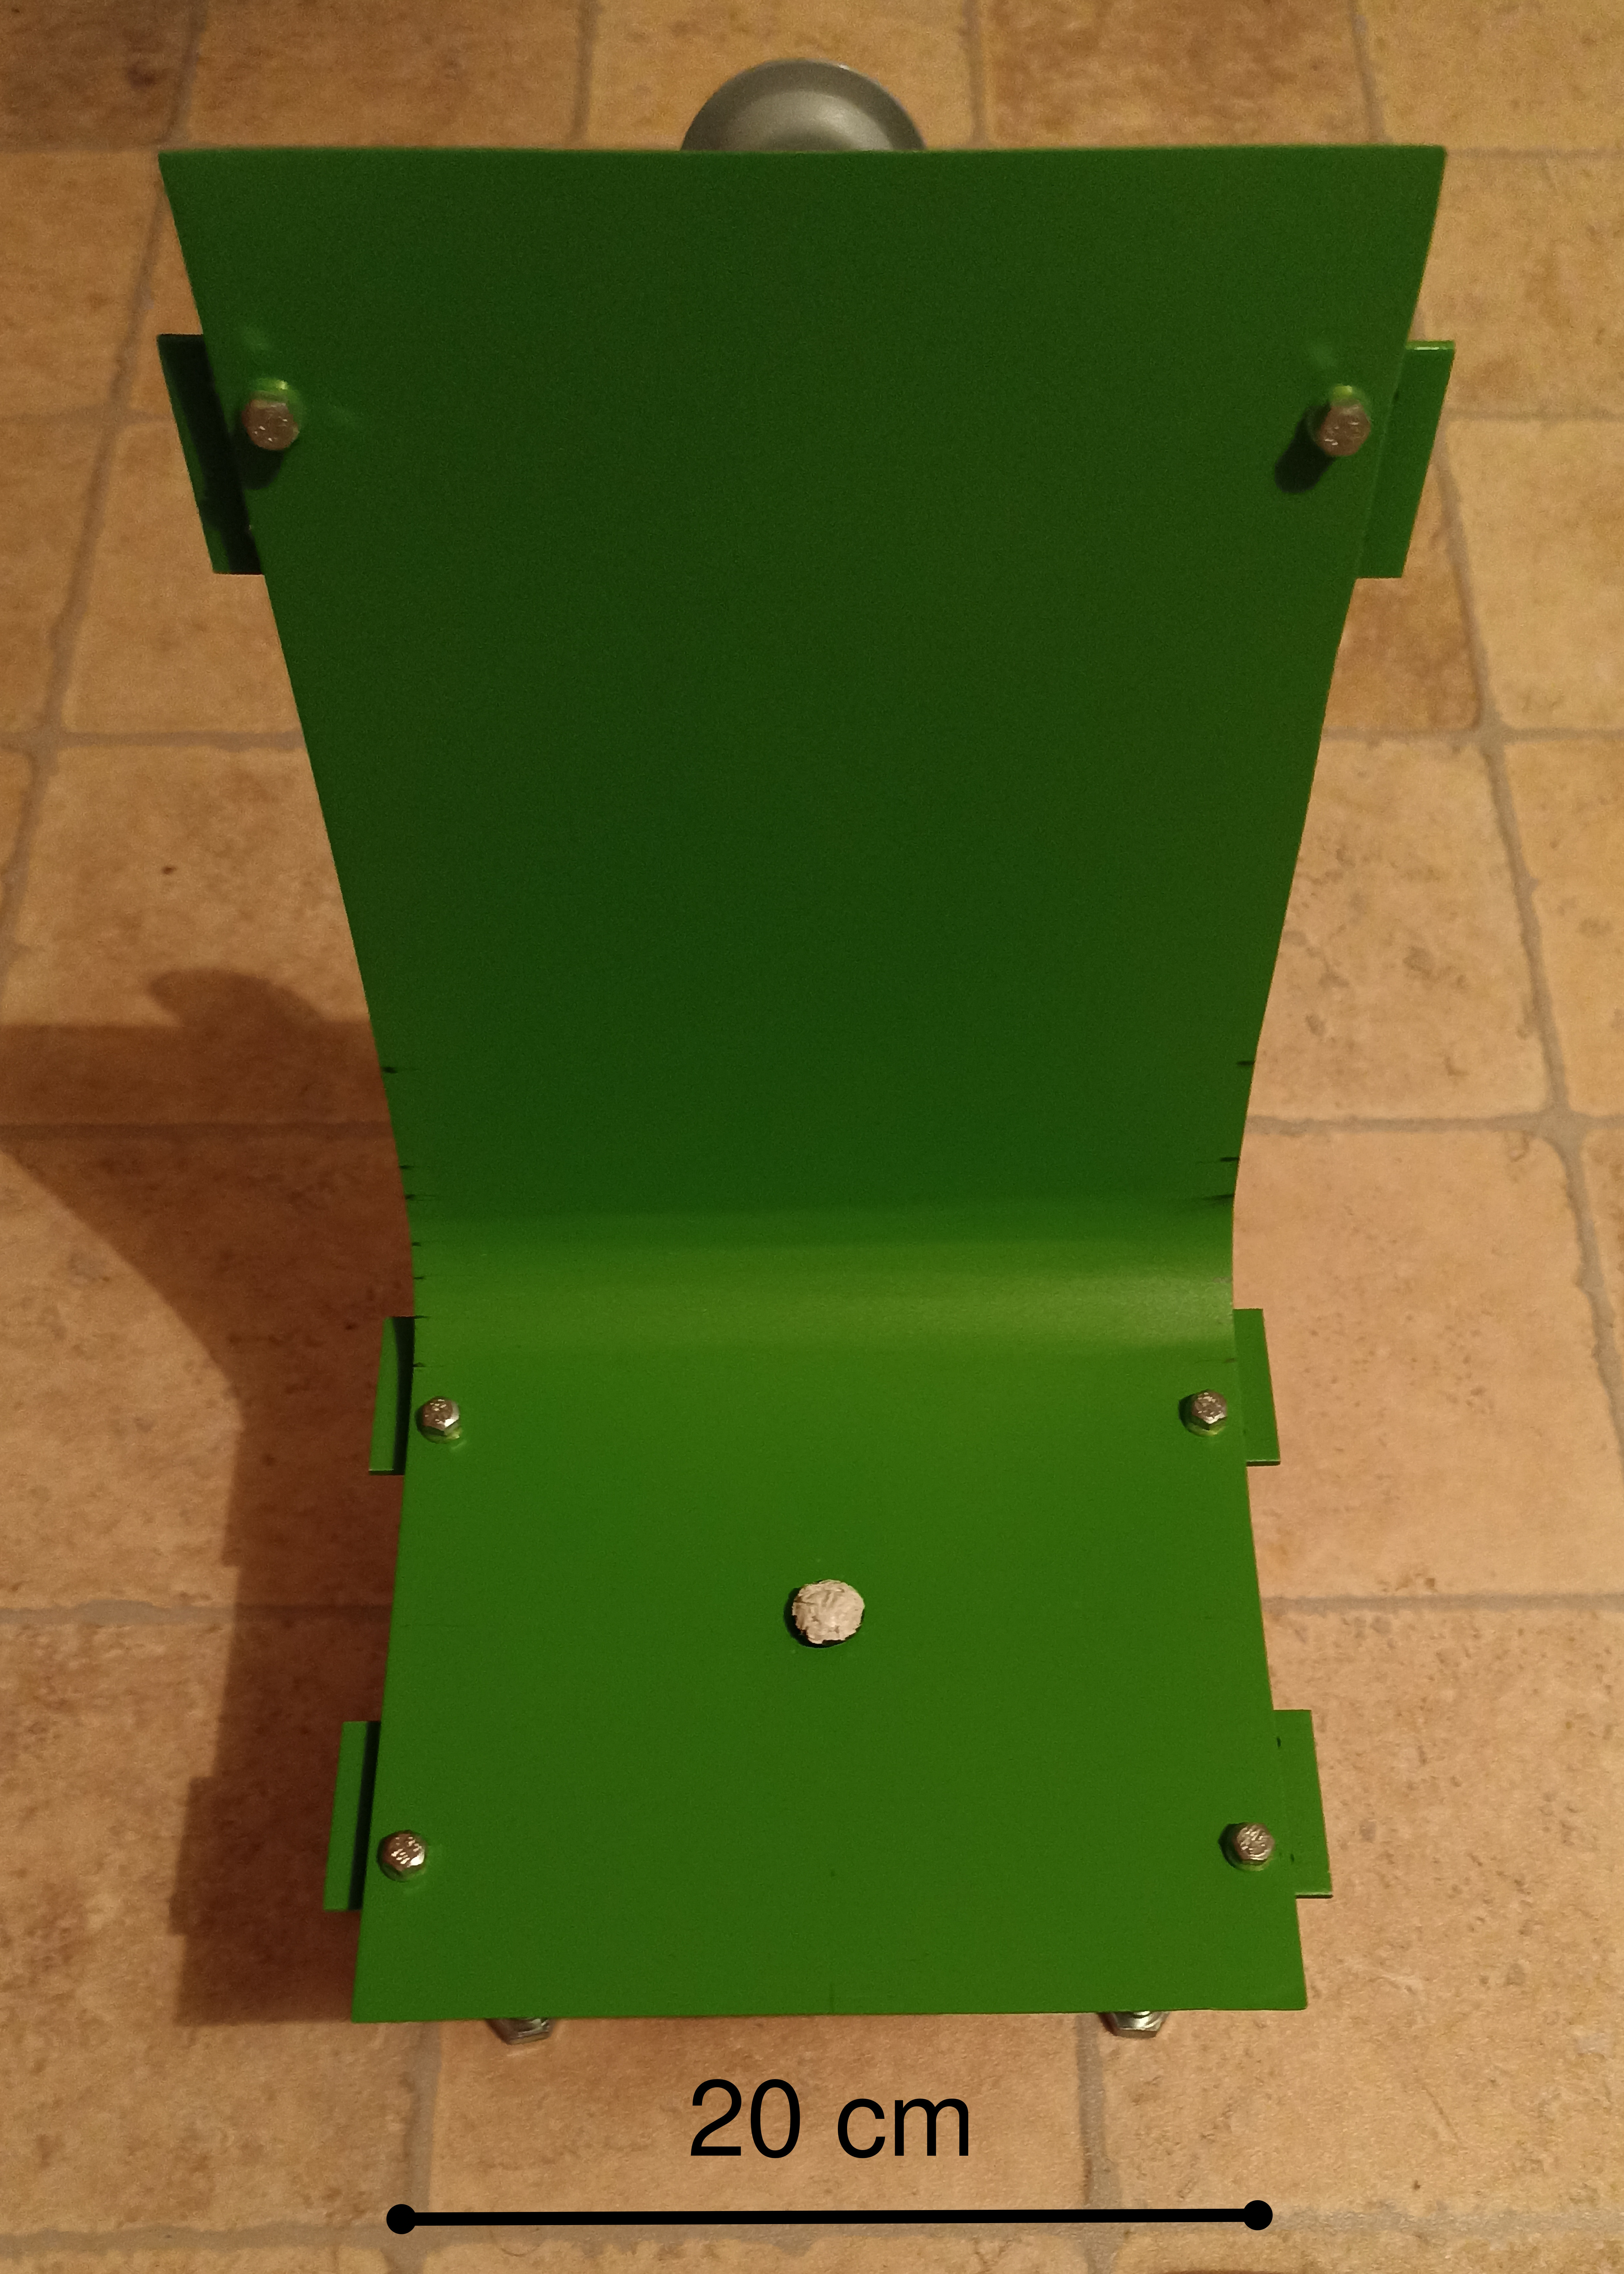
\includegraphics[width=8cm]{images/zpredu.jpg}
                \subcaption{Pohled zpředu}
            \end{subfigure}
            \hfill
            \begin{subfigure}{8cm}
                \centering
                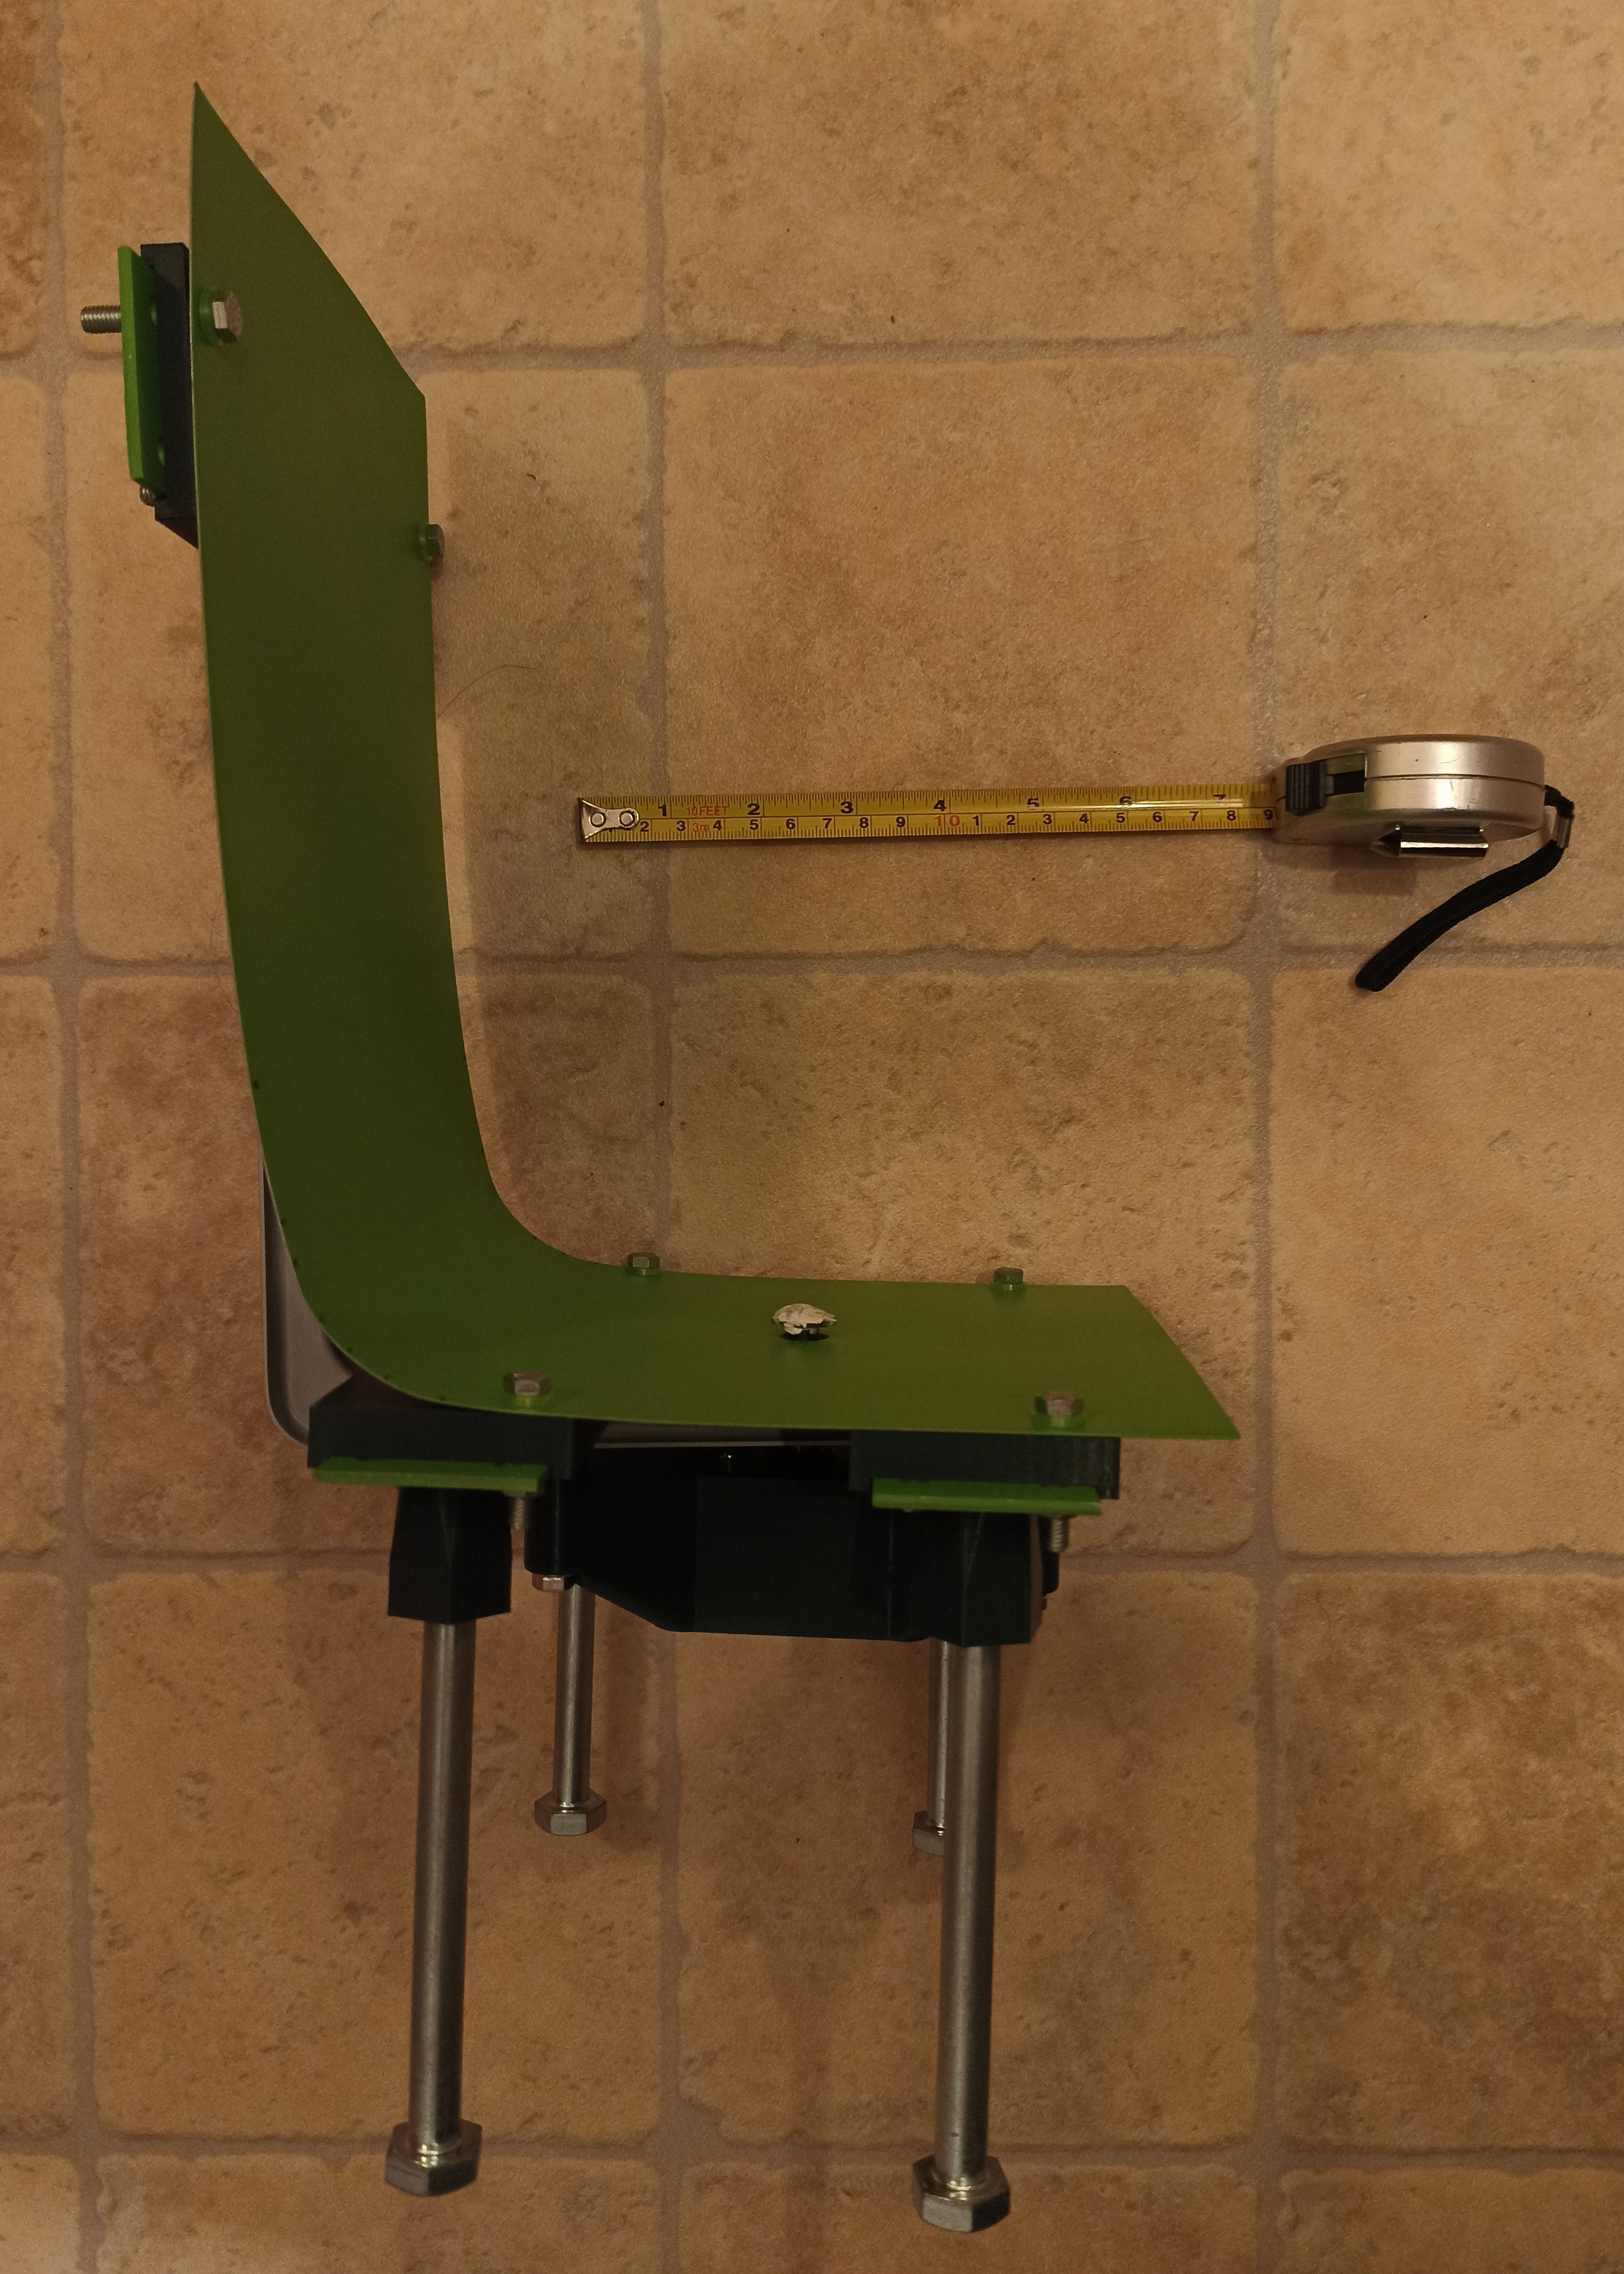
\includegraphics[width =8cm]{images/bok.jpg}
                \subcaption{Pohled zboku}
            \end{subfigure}
            \caption{Složená židlička na skenování}
        \end{figure}

    	\begin{figure}[h]
    	    \centering
    	    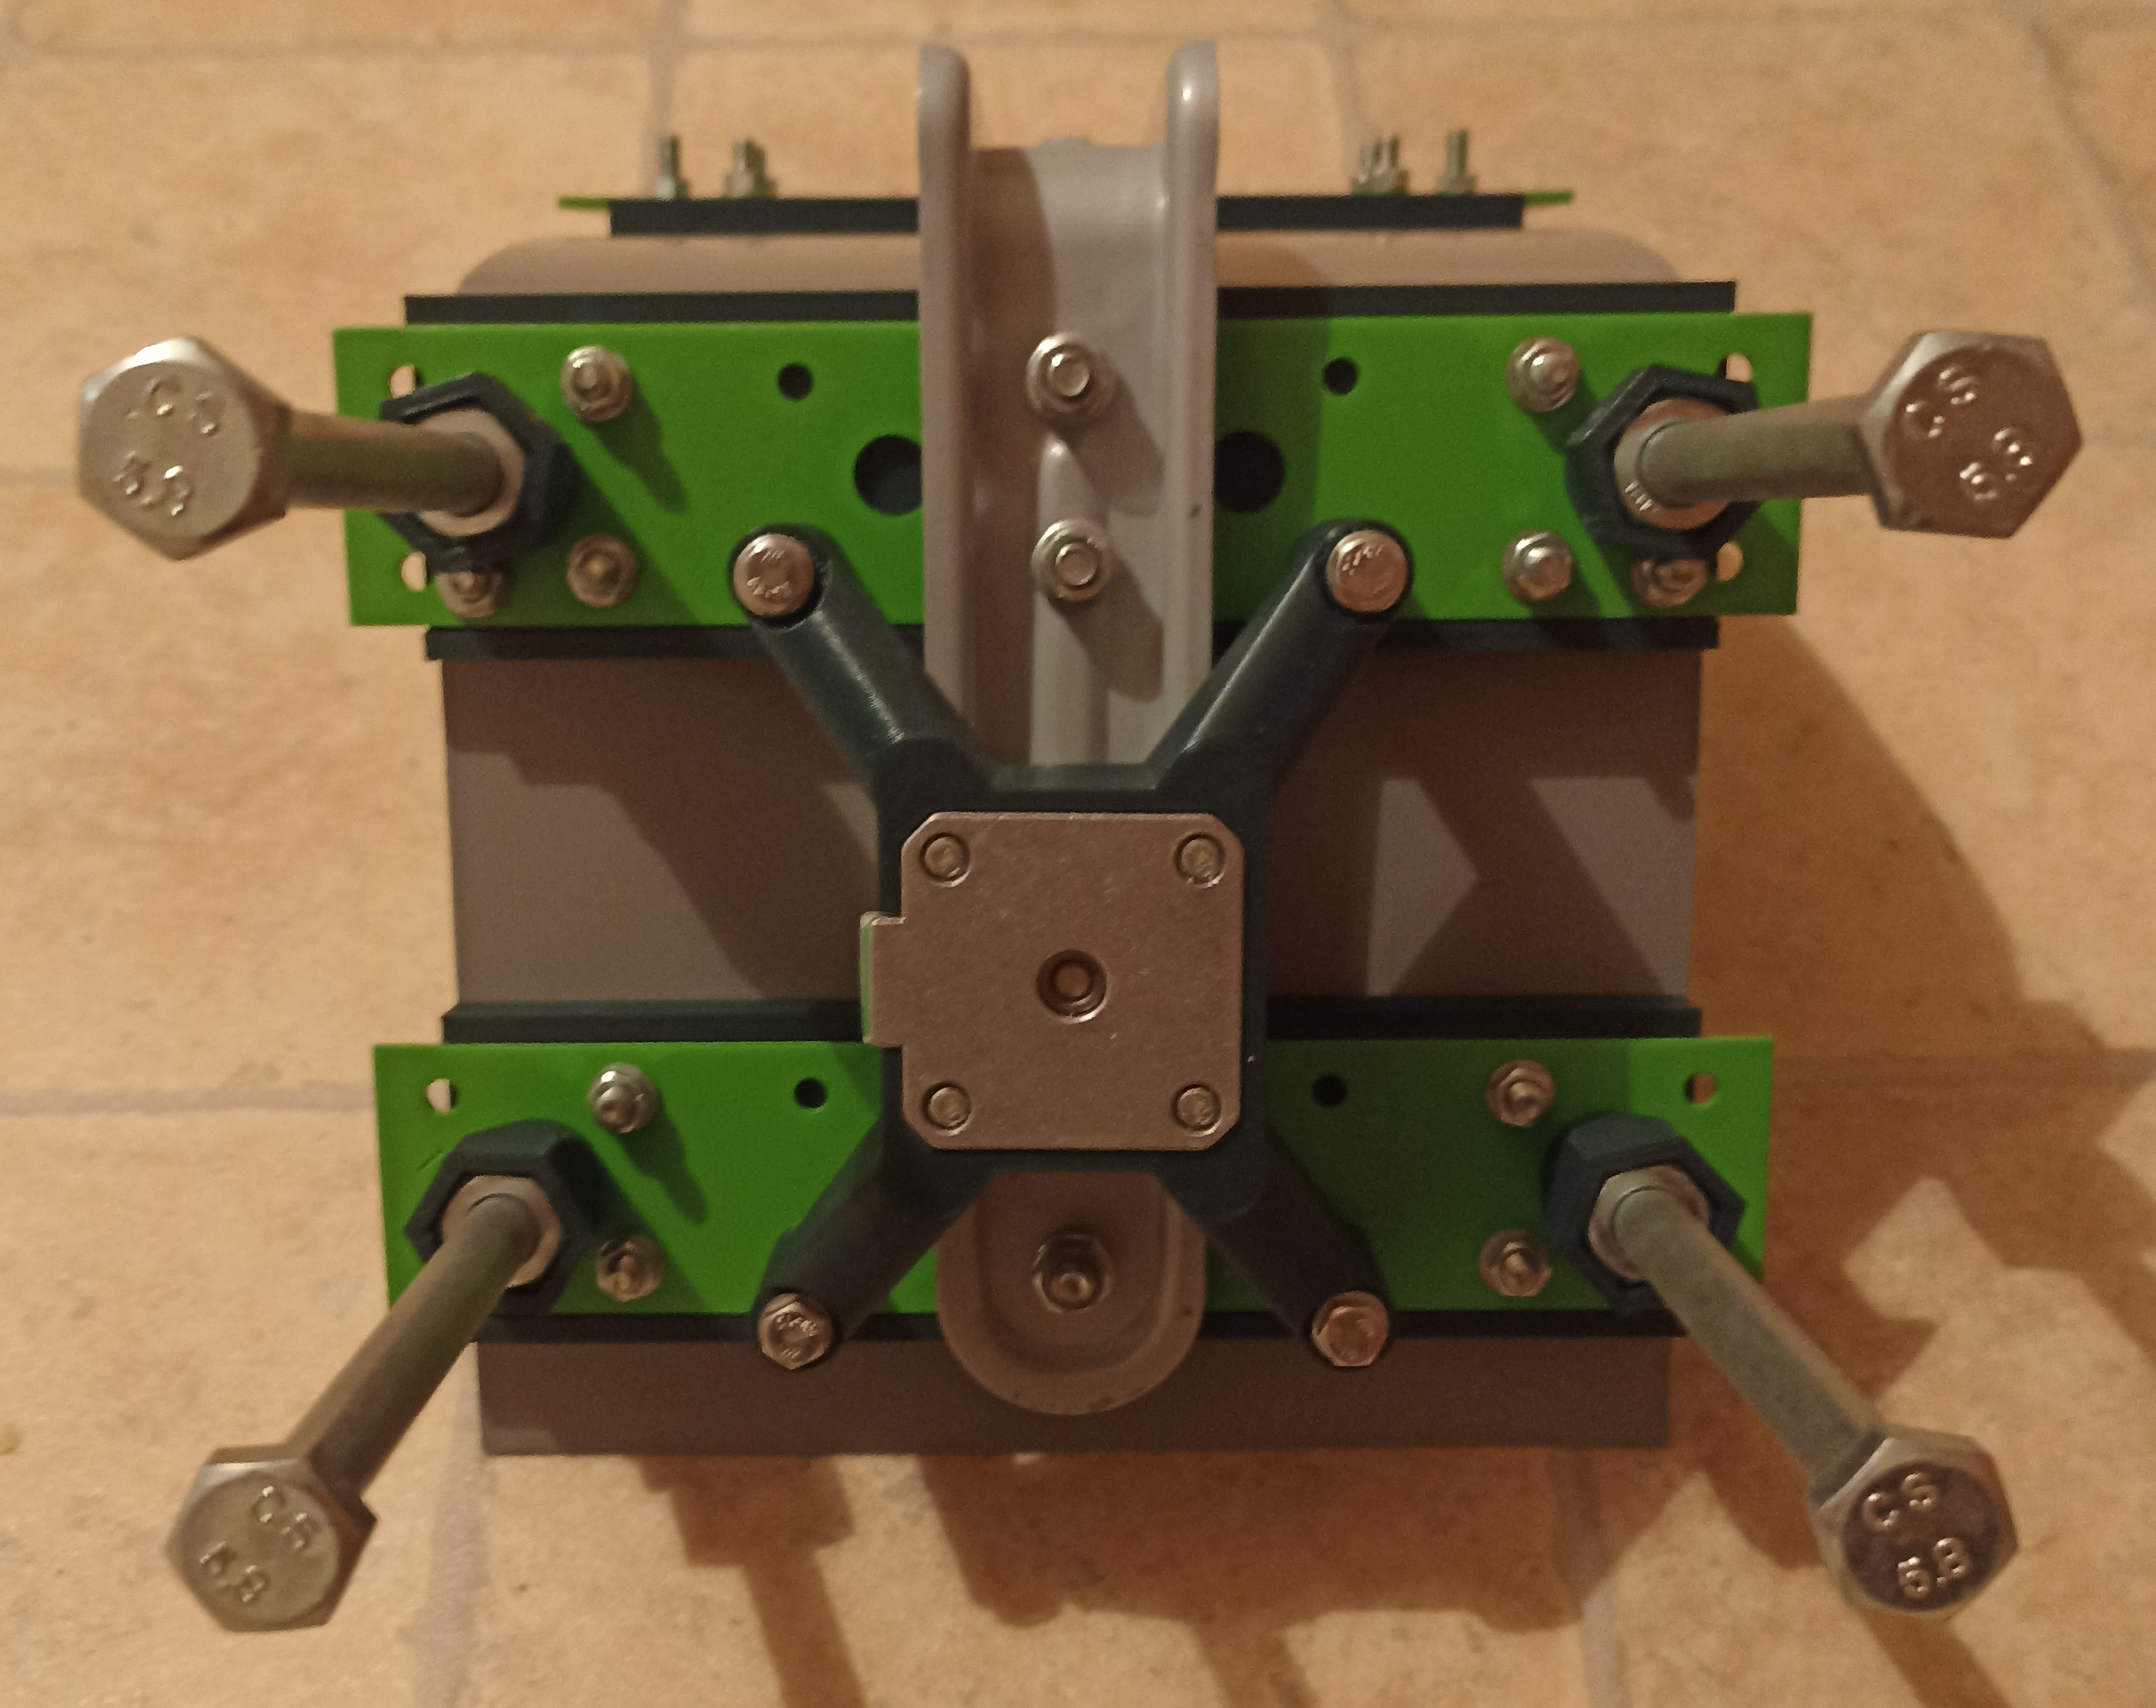
\includegraphics[width=\textwidth]{images/zezpodu.jpg}
    	    \caption{Pohled zdola}
    	\end{figure}

        \begin{figure}[h]
            \centering
            \includegraphics[width =\textwidth]{images/foceniPredmetu.jpg}
            \caption{Focení předmětu na krokovém motoru}
        \end{figure}


    \chapter{Tisk výsledků na Prusa i3 MK3S+}
        \begin{figure}[h]
            \centering
            \includegraphics[width =\textwidth]{images/tisknutiKamene.jpg}
            \caption{Tisk modelu kamene}
        \end{figure}
       
        \begin{figure}[h]
            \centering
            \includegraphics[width =\textwidth]{images/tisknutiKachny.jpg}
            \caption{Tisk modelu gumové kačenky}
        \end{figure}
       
        \begin{figure}[h]
            \centering
            \includegraphics[height=\textwidth, angle = 270]{images/tisknutiSochy.jpg}
            \caption{Tisk modelu dřevěné sošky}
        \end{figure}
       
    \chapter{Srovnání výtisků}
        \begin{figure}[h]
            \centering
            \includegraphics[width =\textwidth]{images/kamenSrovnani.jpg}
            \caption{Porovnání modelu kamene}
        \end{figure}
       
        \begin{figure}[h]
            \centering
            \includegraphics[width =\textwidth]{images/kacenaSrovnani.jpg}
            \caption{Porovnání modelu gumové kačenky}
        \end{figure}
       
        \begin{figure}[h]
            \centering
            \includegraphics[width =\textwidth]{images/sochaPorovnani.jpg}
            \caption{Porovnání modelu dřevěné sošky}
        \end{figure}

    \chapter{Program pro Arduino}
    
        \begin{lstlisting}
# include <Stepper.h>

# define STEPS_PER_REV 200 // count of steps per one revolution
# define SPEED 20
Stepper motor(STEPS_PER_REV, 8,9,10,11);

void setup() {
 Serial.begin(115200);  // beginning of Serial communication
 motor.setSpeed(SPEED);
}
void loop() {
   while (!Serial.available()); // waiting for message
   
   int steps2rotate = Serial.readString().toInt();
   motor.step(steps2rotate);    // rotating the object
   Serial.print(1);     // confirming that object is ready to be photographed

}
        \end{lstlisting}

    \chapter{Program pro komunikaci s~Arduinem a~kamerou}

        \begin{lstlisting}[language=Python]
import serial
import cv2
import time
import numpy as np

PATH = "./imgs"  # where to store photos
SIZE_X=300      # width in px
SIZE_Z=400      # height in px

# range of green in HSV
LOWER_GREEN = np.array([36,71,59])
UPPER_GREEN = np.array([88,255,205])

# beginning of serial communication
arduino=serial.Serial(port='/dev/ttyACM0', baudrate=115200, timeout=None) 
# connection to web cam
cam=cv2.VideoCapture("/dev/video2")


def write(x):
    # sends command to rotate through serial com and waits for confirmation
    # x is number of steps, full revolution = 200 steps
    
    arduino.write(bytes(x, 'utf-8'))
    arduino.read(1) # waiting for response

def storeImg(i):
    # takes a photo and stores it as 'i.pbm/i.ppm'
    
    for j in range(50):
        # repeatedly reading to give time for stabilizing the image
        _,original = cam.read()

    # crop the image
    posunX = (len(original[0])-SIZE_X)//2 
    posunZ = (len(original)-SIZE_Z)//2  
    original = original[posunZ:SIZE_Z+posunZ,posunX:SIZE_X+posunX]

    hsv = cv2.cvtColor(original,cv2.COLOR_BGR2HSV)  # converting to HSV
    rgb = cv2.cvtColor(original,cv2.COLOR_BGR2RGB)  # converting to RGB
    mask=cv2.inRange(hsv, LOWER_GREEN, UPPER_GREEN) # converting to .pbm

    # save PBM
    with open(f"{PATH}/pbm/{i}.pbm", mode="w") as file:
        print(f"P1\n{len(mask[0])}\n{len(mask)}",file=file) # header
        for row in mask: 
            for column in row:
                if(column == np.uint8(255)):
                    print("1",end="",file=file)
                else: print("0",end="",file=file)

    # save PPM
    with open(f"{PATH}/ppm/{i}.ppm", mode="w") as file:
        print(f"P3\n{len(rgb[0])}\n{len(rgb)}\n255",file=file) # header
        for row in rgb:
            for column in row:
                for p in column:
                    print(p, end = " ", file=file)


# 2s time pause and motor test - one rev  to the left, one to the right
time.sleep(2)
write("200")
write("-200")

for i in range(0,100):
    time.sleep(2.5)
    storeImg(i) # taking photo i
    write(str(2)) # rotating 2 steps
        \end{lstlisting}


    \chapter{cloud.h}
        \begin{lstlisting}[language = C++]
#include <math.h>
#include <fstream>
#include <vector>
#include <map>
#include <tuple>
#include <queue>
#include <algorithm>

using namespace std;

struct posFloat{
    float x,y,z;
    float distanceTo(posFloat i){
        return sqrt( pow(i.x-x,2)
                    +pow(i.y-y,2)
                    +pow(i.z-z,2));
    }
};
struct posInt{
    int x,y,z;
    int distanceTo(posInt i){
        return int(sqrt( pow(i.x-x,2)
                        +pow(i.y-y,2)
                        +pow(i.z-z,2))); 
    } 
};
struct color{int r,g,b;};

const vector<posInt>  SITES_INDEXES = {
    {0,-1,0}, {0,1,0}, {1,0,0}, {-1,0,0}, {0,0,-1}, {0,0,1} };
const vector<vector<posFloat> > SITES_VERTICIES={
    {{-.5,-.5,-.5},{ .5,-.5,-.5},{ .5,-.5, .5},{-.5,-.5, .5}},
    {{-.5, .5,-.5},{ .5, .5,-.5},{ .5, .5, .5},{-.5, .5, .5}},
    {{ .5,-.5,-.5},{ .5,-.5, .5},{ .5, .5, .5},{ .5, .5,-.5}},
    {{-.5,-.5,-.5},{-.5,-.5, .5},{-.5, .5, .5},{-.5, .5,-.5}},
    {{-.5,-.5,-.5},{ .5,-.5,-.5},{ .5, .5,-.5},{-.5, .5,-.5}},
    {{-.5,-.5, .5},{ .5,-.5, .5},{ .5, .5, .5},{-.5, .5, .5}}
};

class Point{
    private:
        posFloat pos;   // coordinates of the point
        posFloat smoothVector = {0,0,0};
        int colorPhotosCount = 0;   // how many photos involved in coloring
        color col = {0,0,0};
    public:
        // making some private values readable
        const float& x = pos.x;
        const float& y = pos.y;
        const float& z = pos.z;
        const int& r = col.r;
        const int& g = col.g;
        const int& b = col.b;

        Point(float x, float y, float z){  // constructor
            pos = {x,y,z};
        }

        /* RETURNS DISTANCE TO POINT i */
        float distanceTo(Point* i){
            return pos.distanceTo({i->x,i->y,i->z});
        }        
        
        /* FIRSTLY ROTATES POINT BY angleZ AROUND Z-AXIS, THEN
           BY angleX AROUND X-AXIS, pc IS POSITION OF THE
           ORIGIN OF THE COORDINATE SYSTEM */
        posFloat rotate(posFloat pc, float angleX, float angleZ){
            angleX *= M_PI/180; // to radians
            angleZ *= M_PI/180;
            posFloat trnsfrm;
            // around z
            trnsfrm.x = (pos.x-pc.x)*cos(angleZ) + (pos.y-pc.y)
                        * sin(angleZ) + pc.x;
            trnsfrm.y = (pc.x - pos.x)*sin(angleZ) + (pos.y-pc.y)
                        * cos(angleZ) + pc.y;
                        
            // around x
            trnsfrm.z = (pos.z-pc.z)*cos(angleX) + (trnsfrm.y-pc.y)
                        * sin(angleX) + pc.z;
            trnsfrm.y = (pc.z-pos.z)*sin(angleX) + (trnsfrm.y-pc.y) 
                        * cos(angleX) + pc.y;
            
            return trnsfrm;
        }

        /* RETURNS POSITION OF THE PROJECTED POINT IN PHOTO */
        pair<int,int> project(posFloat pc, posFloat cam, posInt size,
                              float angleX, float angleZ){
            
            posFloat pos = rotate(pc,angleX,angleZ);
            pos.x = cam.x +(cam.y/(cam.y-pos.y)*(pos.x-cam.x));
            pos.z = cam.z +(cam.y/(cam.y-pos.y)*(pos.z-cam.z));
            
            // calibration of the axis shift relative to the center of the photo
            pos.x += size.x/2-cam.x;
            pos.z += size.z/2-cam.z;
            return {pos.x, pos.z};
        }

        /* ADDS THE VECTOR TO THE NEIGHBOR TO FORM THE RESULTING smoothVector,  v IS THE END POINT OF THE VECTOR, THE STARTING POINT IS THE CALLED ONE */
        void addSmoothVector(Point* v){ 
            smoothVector.x += v->x-pos.x;
            smoothVector.y += v->y-pos.y;
            smoothVector.z += v->z-pos.z;
        }
        void moveBySmoothVector(){
            const int SMOOTH_COEFICIENT = 100;
            pos.x += smoothVector.x/SMOOTH_COEFICIENT;
            pos.y += smoothVector.y/SMOOTH_COEFICIENT;
            pos.z += smoothVector.z/SMOOTH_COEFICIENT;
        }
        void resetSmoothVector(){
            smoothVector = {0,0,0};
        }
        void add2AverageColor(color c){
            col.r += c.r;
            col.g += c.g;
            col.b += c.b;
            colorPhotosCount++; // from how many photos the average point color is calculated 
        }
        /* COMPLETING THE AVERAGE COLOR CALCULATION */
        void setAverageColor(){
            if(colorPhotosCount==0) return;
            col.r = col.r/colorPhotosCount;
            col.g = col.g/colorPhotosCount;
            col.b = col.b/colorPhotosCount;
        }
};

class PBMphoto{
    private:
        vector<vector<bool> > img; // 2D array of pixels
        int sizeX, sizeY;
    public:
        PBMphoto(string path){ // reading photo from 'path'
            ifstream fin(path);
            string header;
            fin>> header >> sizeX >> sizeY;
            img.resize(sizeY, vector<bool>(sizeX));

            bool pixel;
            for (int y = sizeY-1; y>=0; y--)
                for(int x = sizeX-1; x>=0;x--){
                bool pixel;
                fin >> pixel;
                img[y][x]=pixel;   
            }
        }
        /* RETURNS PIXEL VALUE */
        bool getBitValue(int x, int y){
            if(x < 0 || x > sizeX-1 || y < 0 || y > sizeY-1) return 0;
            return img[y][x];
        }
};


class PPMphoto{ 
    private:
        vector<vector<color> > img; // array of pixels
        int sizeX; int sizeY;
    public:
        PPMphoto(string path){ // reading photo from 'path'
            ifstream fin(path);
            string header, maxVal;
            fin>>header >> sizeX >> sizeY >> maxVal;
            
            img.resize(sizeY);
            for(vector<color>& y : img) y.resize(sizeX);

            color pixel;
            for (int y = sizeY-1; y>=0; y--)
                for(int x = sizeX-1; x>=0;x--){
                    fin >> pixel.r >> pixel.g >> pixel.b;
                    img[y][x] = pixel;
                }
          
        }
        /* RETURNS PIXEL COLOR */
        color getBitValue(int x, int y){
             if(x < 0 || x > sizeX-1 || y < 0 || y > sizeY-1)
                return {0,0,0};
             return img[y][x];
         }
};


class Cloud{
private:
/*  PRIVATE VARIABLES
* size -> size of the cloud
* cubes -> list of the centers of the cubes the cloud is
           consisted of
* pointCloudModel -> 3D array for cloud visualization
* mp -> maps coordinates to vertex index
* verticies -> list of verticies of the mesh
* faces -> list of indexes of verticies, contains only
           tetragons, verticies of a tetragon are at
           {faces[4k],faces[4k+1],faces[4k+2],faces[4k+3]}
*/

    posInt size;
    queue<Point*> cubes;
    vector<vector<vector<bool> > > pointCloudModel;
    map<tuple<float,float,float>, int> mp;
    vector<Point*> verticies;
    vector<int> faces;
       
public:

    /* WHEN CONSTRUCTING THE CLOUD */
    Cloud(int sizeX, int sizeY, int sizeZ){
        size={sizeX, sizeY, sizeZ};
       
        // creating points and pushing them to 'cubes'
        for(int ix = 0; ix < size.x; ix++)
            for(int iy = 0; iy < size.y; iy++)
                for(int iz = 0; iz < size.z; iz++){
                    Point* pointerP = new Point(ix,iy,iz);
                    cubes.push(pointerP);
                }
        // resizing pointCloudModel
        pointCloudModel.resize(size.x);
        for (vector<vector<bool> >& v : pointCloudModel)
            v.resize(size.y, vector<bool>(size.z,false));
    }

    /* CROPS CLOUD BASED ON THE PHOTO AT THE ADDRESS OF
       'picture' */
    void crop(string picture, posFloat camera,
              posFloat center, float angleZ, float angleX){
        
        PBMphoto img(picture);

        // pushing separator into the queue
        Point* sep = new Point(-1,-1,-1);
        cubes.push(sep);
        
        // iterating through cubes until separator shows up
        while(cubes.front()!=sep){ 
            pair<int,int> fotoPos = cubes.front()->project(
                         center,camera,size,angleX,angleZ); 
            if(img.getBitValue(fotoPos.first,
               fotoPos.second))cubes.push(cubes.front());
            
            cubes.pop();
        }
        cubes.pop(); // popping separator 
    }
    /* MARKS ACTIVE CUBES IN POINTCLOUDMODEL */
    void markPTM(){
        Point* sep = new Point(-1,-1,-1);
        cubes.push(sep); // pushing separator

        // iterating through cubes
        while(cubes.front()!=sep){
            Point* p = cubes.front();
            pointCloudModel[p->x][p->y][p->z]=true;
            cubes.pop();
        }
        cubes.pop();   // popping separator
    }

    /* ARE THE COORDINATES INSIDE THE CLOUD? */
    bool isIn(posInt pos){
        if (pos.x < 0) return false;
        if (pos.x >= size.x) return false;
        if (pos.y < 0) return false;
        if (pos.y >= size.y) return false;
        if (pos.z < 0) return false;
        if (pos.z >= size.z) return false;
        return true;
    }

    /* HOW MANY NEIGHBOR CUBES HAVE THE OPPOSITE VALUE,
       NEIGHBORS SHARE A FACE! */ 
    int countOpositNeighbours(posInt where){
        int count = 0;
        for(int i = 0; i < 6; i++){
            posInt n ={ where.x+SITES_INDEXES[i].x,
                            where.y+SITES_INDEXES[i].y,
                            where.z+SITES_INDEXES[i].z
                          };
            
            if (isIn(n) &&
                !pointCloudModel[n.x][n.y][n.z] == 
                pointCloudModel[where.x][where.y][where.z])
                    count+=1;
                
        }
        return count;
    }

    /* REMOVES TRASH */
    void solveSingleCubes(){
        for (int ix = 0; ix < size.x; ix++)
            for (int iy = 0; iy < size.y; iy++)
                for (int iz = 0; iz < size.z; iz++){
                    posInt where;
                    where.x = ix; where.y = iy; where.z = iz;
                    if(countOpositNeighbours(where)>=5)
                        pointCloudModel[ix][iy][iz] = !pointCloudModel
                                                         [ix][iy][iz];
                }
    }

    /*ITERATING OVER POINTCLOUDMODEL, DETECTING CUBES ON THE SURFACE OF THE OBJECT, WRITING VERITICIES AND FACES INTO THEIR ARRAYS*/
    void findFaces(){
        int currentIndex = 0;   
        markPTM();
        solveSingleCubes();

        /* for every highlighted (val = true) cube look at its neighbors, 
           if neighbor is unhighlighted (val = false), the face they share
           must be a part of the mesh, mp maps coordinates to index of
           a vertex which helps us avoid having duplicates in 
           the 'verticies' array
        */ 
        for (int ix = 0; ix < size.x; ix++)
           for (int iy = 0; iy < size.y; iy++)
              for (int iz = 0; iz < size.z; iz++) 
                 if (pointCloudModel[ix][iy][iz])
                    for(int i = 0; i < 6; i++){
                        posInt neighbour = {ix+SITES_INDEXES[i].x,
                                            iy+SITES_INDEXES[i].y,
                                            iz+SITES_INDEXES[i].z};
            
                  if(!isIn(neighbour) || !pointCloudModel 
                     [neighbour.x][neighbour.y][neighbour.z])
                        for (posFloat bod : SITES_VERTICIES[i]){
                          posFloat p = {bod.x+ix,bod.y+iy,bod.z+iz}; 
                                
                          if(mp.find({p.x,p.y,p.z})==mp.end()){
                              mp.insert({{p.x,p.y,p.z}, currentIndex});
                              verticies.push_back(new Point(p.x,p.y,p.z));
                              currentIndex++;
                          }
                          faces.push_back(mp.find({p.x,p.y,p.z})->second);
                        }
            }
    }

    /* SETS A SMOOTHVECTOR TO EVERY VERTEX */
    void setSmoothVectors(){
        for(int i = 0; i < faces.size(); i += 4)
            for(int j = 0; j < 4; j++){
              verticies[faces[i+j]]->
              addSmoothVector(verticies[faces[i+(j+1)%4]]);
                
              verticies[faces[i+j]]->
              addSmoothVector(verticies[faces[i+(j+3)%4]]);
            }
    }


    /* MAKES THE MESH SMOOTHER*/
    void smoothMesh(){
        for(Point* p : verticies)
            p->resetSmoothVector();
        setSmoothVectors();
        for(Point* p : verticies)
            p->moveBySmoothVector();
    }

    /* ADDS TEXTURE BASED ON PHOTO FROM 'source' */
    void color(string source, posFloat camera,
              posFloat center, float angleX, float angleZ){

        vector<vector<vector<pair<Point*,int> > > > grid;
        grid.resize(size.z, vector<vector<pair<Point*,int> > >(size.x));

        /* sorting verticies into grid */
        for (Point* v : verticies){
          pair<int,int> where = v->project(
            center,camera,size,-angleX,angleZ*(-3.6));
          if(where.first>=0 && where.first<size.x &&
          where.second>=0 && where.second<size.z){
            posFloat rotated = v->rotate(center,-angleX,angleZ*(-3.6));
            int dist = rotated.distanceTo(camera);
            // the nearest point is always in the first place
            if(!grid[where.second][where.first].empty() &&
            dist < grid[where.second][where.first][0].second){
                grid[where.second][where.first].push_back(
                    grid[where.second][where.first][0]);
                grid[where.second][where.first][0]={v,dist};
            } 
            else
            grid[where.second]
                [where.first].push_back({v,dist});

          }
        }

        PPMphoto photo(source);
        /* going through the pixels of the photo and deciding based on the distance whether the points will be colored or not */
        for (int i = 2; i < size.z - 2; i++)
            for(int j = 2; j < size.x - 2; j++)
                if(!grid[i][j].empty()){
                    int nearest = grid[i][j].front().second;
                    for(int a : {-2,-1,1,2}) for(int b : {-2,-1,1,2})
                        if(!grid[i+a][j+b].empty())
                            nearest = min(nearest, grid[i+a][j+b].front().
                                                                  second);
                for (pair<Point*,int> v : grid[i][j])
                    if (v.second-nearest < 6)
                        v.first->add2AverageColor(photo.getBitValue(j,i));
            }
    
    }

    /* OBJECT IS SAVED IN PLY FORMAT */
    void writeMesh(string address){
        ofstream fout(address);

        for (Point* p: verticies) // finishing point coloring
            p->setAverageColor();

        // header
        fout << "ply\n";
        fout << "format ascii 1.0\n";
        fout << "comment author: Martin Cerveny\n";
        fout << "element vertex "<< verticies.size() << endl;
        fout << "property float x\n";
        fout << "property float y\n";
        fout << "property float z\n";
        fout << "property uchar red\n";
        fout << "property uchar green\n";
        fout << "property uchar blue\n";
        fout << "element face " << faces.size()/4 << endl;
        fout << "property list uchar uint vertex_indices\n";
        fout << "end_header\n"; 

        // list of verticies
        for(Point* p : verticies)
            fout << p->x << " " << p->y << " " << p->z <<" "<< p->r << " " << p->g <<" "<< p->b << endl;
        
        // list oof faces
        for(int i = 0; i < faces.size(); i+=4){   
            fout << "4";
            for(int j = 0; j < 4; j++)
                fout << " " << faces[i+j];
            fout << endl;
        }
    }
   
};

        \end{lstlisting}

    \chapter{main.cpp}
        \begin{lstlisting}
#include<iostream>
#include<fstream>
#include"cloud.h"

using namespace std;

int main(){

    const string IMGSOURCE = "./imgs/duck/";
                           //"./imgs/sculpture/";
                           //"./imgs/stone/";

    /* getting size info */
    ifstream inSize(IMGSOURCE+"/cloudSize");
    int sizeX, sizeY, sizeZ; inSize >> sizeX >> sizeY >> sizeZ;

    /* creating cloud */
    Cloud c(sizeX,sizeY,sizeZ);

    /* cropping */
    for(int series : {12,40}){
        ifstream inCalib(IMGSOURCE+to_string(series)+"/calib");
        float cameraX,cameraY,cameraZ,centerX,centerY,centerZ;
        inCalib>>cameraX>>cameraY>>cameraZ>>centerX>>centerY
               >>centerZ;
        for (int i = 0 ; i < 25;i++){
            for (int j : {0,25,50,75}){
                int photo = i + j;
                string path = IMGSOURCE+to_string(series)
                              +"/pbm/"+to_string(photo)+".pbm"; 
                c.crop(path, {cameraX, cameraY, cameraZ},
                       {centerX, centerY, centerZ},
                       -3.6*(photo), -series);
            }
            cout << series << ":[" << 4*i << "%]\n";
        }
    }
    cout << "cloud cropped" << endl;
    c.findFaces();
    cout << "mesh created" << endl;
    for(int i = 0; i < 300; i++)
       c.smoothMesh();
    cout << "model smoothed" << endl;

    cout << "coloring" << endl;
    for (int i = 0; i < 100; i++)
      for(int series : {12,40}){
        ifstream inCalib(IMGSOURCE+to_string(series)+"/calib");
        float cameraX,cameraY,cameraZ,centerX,centerY,centerZ;
        inCalib>>cameraX>>cameraY>>cameraZ>>centerX>>centerY
               >>centerZ;
           
        string source = IMGSOURCE+to_string(series)+"/ppm/"+
                        to_string(i)+".ppm";
        c.color(source, {cameraX, cameraY, cameraZ},{centerX,
                centerY, centerZ}, series,i);
        
        }
    cout << "texture added" << endl;

    c.writeMesh(IMGSOURCE+"model.ply");
    cout << "done" << endl;

    return 0;    
}
        \end{lstlisting}


\end{appendices}

\end{document}
